\documentclass[a4paper,12pt, twoside]{scrreprt}
% Autor der Vorlage: Klaus Rheinberger, FH Vorarlberg
% 2017-02-20

%% Hilfe: z.B.
% empfohlener Einstieg: http://latex.tugraz.at/  
% https://de.wikibooks.org/wiki/LaTeX-Kompendium:_Schnellkurs:_Erste_Schritte
% https://de.wikibooks.org/wiki/LaTeX-Kompendium:_Schnellkurs
% https://de.wikibooks.org/wiki/LaTeX-Kompendium

%% Pakete:
% Der Befehl \usepackage[latin9]{inputenc} ermöglicht die direkte Angabe von Umlauten. Übrigens lässt sich so auch das Euro-Zeichen direkt eingeben. Auf Betriebssystemen, wie zum Beispiel allen neueren Linux-Distributionen, verwendet man statt \usepackage[latin9]{inputenc} besser \usepackage[utf8]{inputenc}, auf Applesystemen verwendet man \usepackage[macce]{inputenc} (oder das für ältere Modelle gültige \usepackage[applemac]{inputenc}).
\usepackage[utf8]{inputenc}
\usepackage[T1]{fontenc}    % Silbentrennung bei Sonderzeichen
\usepackage{graphicx}       % Bilder einbinden
\usepackage[ngerman]{babel} % Deutsche Sprachanpassungen
\usepackage{csquotes}       % When using babel or polyglossia with biblatex, loading csquotes is recommended to ensure that quoted texts are typeset according to the rules of your main language.
\usepackage{acronym}  % für optionales Abkürzungsverzeichnis
\usepackage{eurosym}  % z. B. \EUR{12345,68}
\usepackage[linktocpage=true]{hyperref} % Links z. B. \href{https://www.wikibooks.org}{Wikibooks home}
\usepackage{caption} % Abbildungslegenden
\captionsetup{format=hang, justification=raggedright}
%\usepackage[style=alphabetic,citestyle=alphabetic,backend=bibtex]{biblatex}   % Literaturverweise

%% own packages
\usepackage{longtable}
\usepackage{ragged2e}
\usepackage[german]{datetime2}
\usepackage{listings}
\usepackage[style=alphabetic,citestyle=alphabetic,backend=bibtex,block=ragged]{biblatex}
\addbibresource{bibresource.bib}

\usepackage{color}
%\usepackage[dvipsnames]{xcolor}
\usepackage[table, dvipsnames]{xcolor}
\usepackage{paralist}
\usepackage{svg}
\usepackage{enumitem}
\usepackage{listings}
\usepackage[section]{placeins}
%Zitate
%\usepackage[superscript]{cite}
%\usepackage[numbers,round]{natbib}
\usepackage{diagbox}
\usepackage{tcolorbox}
\usepackage[T1]{fontenc}
\usepackage[utf8]{inputenc}
\usepackage{newunicodechar}
\usepackage{siunitx}
\sisetup{locale = DE}

\usepackage{tikz}
\usetikzlibrary{trees, shapes, arrows}

\usepackage{tabularx}
\usepackage{makecell}
\renewcommand\theadfont{\bfseries\sffamily}
\usepackage{xspace}

%\usepackage{multirow}
%\usepackage{booktabs}


\hyphenchar\font=\string"7F
\hyphenation{Online-Programmier-verfahren Be-schleu-ni-gung}

%setup pdf
\hypersetup{
	pdfauthor={Helmut Rhomberg}
	pdfkeywords={Bachelorarbeit, FHV, Node.js, Programmieren, Software Engineer, BSc, Mobile Apps, Server}
	pdftitle={Node.js als Server-Plattform für mobile Apps}
}

\definecolor{bluekeywords}{rgb}{0.13,0.13,1}
\definecolor{greencomments}{rgb}{0,0.5,0}
\definecolor{redstrings}{rgb}{0.9,0,0}
\setcounter{secnumdepth}{4}
\setcounter{tocdepth}{4}   % Tiefe der Gliederung im Inhaltsverzeichnis

% http://latexcolor.com/
% https://en.wikibooks.org/wiki/LaTeX/Colors

\definecolor{lightgray}{rgb}{.9,.9,.9}
\definecolor{darkgray}{rgb}{.4,.4,.4}
\definecolor{purple}{rgb}{0.65, 0.12, 0.82}

\lstdefinelanguage{JavaScript}{
	keywords={break, case, catch, continue, debugger, default, delete, do, else, false, finally, for, function, if, in, instanceof, new, null, return, switch, this, throw, true, try, typeof, var, void, while, with},
	morecomment=[l]{//},
	morecomment=[s]{/*}{*/},
	morestring=[b]',
	morestring=[b]",
	ndkeywords={class, export, boolean, throw, implements, import, this},
	keywordstyle=\color{blue}\bfseries,
	ndkeywordstyle=\color{darkgray}\bfseries,
	identifierstyle=\color{black},
	commentstyle=\color{purple}\ttfamily,
	stringstyle=\color{red}\ttfamily,
	sensitive=true
}

% hypenations
\hyphenation{Kos-ten-er-spar-nis-sen}
\hyphenation{An-wen-dung}

\captionsetup{justification=centering}


%% Einstellungen:
\setcounter{secnumdepth}{4}
\setcounter{tocdepth}{4}   % Tiefe der Gliederung im In haltsverzeichnis

% own macros

\newcommand{\acronymContainer}[1]{
	\begin{flushleft}
		\begin{longtable}{p{0.2\textwidth} p{0.8\textwidth}}
		#1
		\end{longtable}
	\end{flushleft}
}

\newcommand{\acronymEntry}[2]{
	\textbf{#1} & #2
}

\newcommand{\acronymEntryNewline}[0]{
	\vspace*{0.631em} \\
}

\newcommand{\todayWithoutDay}{\DTMlangsetup[german]{showdayofmonth=false}\today\DTMlangsetup[german]{showdayofmonth=true}}

\newcommand{\quoteMark}[1]{%
	\glqq#1\grqq%
}

\newcommand{\setCSharpListing}{
	\lstset{language=[Sharp]C,
		extendedchars=\true,
		escapeinside=``,
		inputencoding={utf8},
		showspaces=false,
		showtabs=false,
		breaklines=true,
		showstringspaces=false,
		breakatwhitespace=true,
		escapeinside={(*@}{@*)},
		commentstyle=\color{greencomments},
		keywordstyle=\color{bluekeywords}\bfseries,
		stringstyle=\color{redstrings},
		basicstyle=\ttfamily,
		captionpos=t
	}
}

\newcommand{\setBashListing}{
	\lstset{language=bash,caption={bash version},
		extendedchars=\true,
		escapeinside=``,
		inputencoding={utf8},
		basicstyle=\ttfamily,
		showstringspaces=false,
		commentstyle=\color{red},
		keywordstyle=\color{blue},
		captionpos=t
	}
}

\newcommand{\setJavaScriptListing}{
	\lstset{language=JavaScript,
		extendedchars=\true,  
		escapeinside=``,
		inputencoding={utf8},
		extendedchars=true,
		basicstyle=\footnotesize\ttfamily,
		showstringspaces=false,
		showspaces=false,
		numberstyle=\footnotesize,
		numbersep=9pt,
		tabsize=2,
		breaklines=true,
		showtabs=false,
		captionpos=t
	}
}

\newcommand{\bracketText}[1]{%
    \textit{\scriptsize{#1}}%
}

% gender some words with macros

\newcommand{\entwicklerSi}{Entwickler}
\newcommand{\entwicklerinSi}{Entwicklerin}
\newcommand{\entwicklerPl}{Entwickler}
\newcommand{\entwicklerinPl}{Entwicklerinnen}
%\newcommand{\EntwicklerSi}{\entwicklerSi{}/\entwicklerinSi{}}
\newcommand{\EntwicklerSi}{\entwicklerinSi{}}
%\newcommand{\EntwicklerPl}{\entwicklerPl{}/\entwicklerinPl{}}
\newcommand{\EntwicklerPl}{\entwicklerinPl{}}
%\newcommand{\demEntwickler}{dem \entwicklerSi{}/der \entwicklerinSi{}}
\newcommand{\demEntwickler}{der \entwicklerinSi{}}
%\newcommand{\denEntwickler}{den \entwicklerSi{}/die \entwicklerinSi{}}
\newcommand{\denEntwickler}{die \entwicklerinSi{}}
%\newcommand{\derEntwickler}{der \entwicklerSi{}/die \entwicklerinSi{}}
\newcommand{\derEntwickler}{der \entwicklerinSi{}}
\newcommand{\desEntwicklers}{des \entwicklerSi{}s}
\newcommand{\dieEntwickler}{die \entwicklerinPl{}}

% to avoid an issue
\newcommand{\dieEntwicklerin}{die \entwicklerinSi{}}

\newcommand{\mitarbeiterSi}{Mitarbeiter}
\newcommand{\mitarbeiterinSi}{Mitarbeiterin}
\newcommand{\mitarbeiterPl}{Angestellten}
\newcommand{\derMitarbeiterPl}{der \mitarbeiterPl{}}

%\newcommand{\benutzerSi}{Anwendende}
\newcommand{\benutzerSi}{User}
%\newcommand{\benutzerPl}{Anwendenden}
\newcommand{\benutzerPl}{User}
\newcommand{\derBenutzer}{der \benutzerSi{}}
\newcommand{\DerBenutzer}{Der \benutzerSi{}}
\newcommand{\einenBenutzer}{einen \benutzerSi}
\newcommand{\desBenutzers}{des \benutzerSi s}
\newcommand{\denBenutzer}{den \benutzerSi}
\newcommand{\demBenutzer}{dem \benutzerSi}
\newcommand{\DemBenutzer}{Dem \benutzerSi}

\newcommand{\ingenieurSi}{diplomierte technische Fachkraft}
\newcommand{\ingenieurPl}{diplomierten technischen Fachkräften}
\newcommand{\vondenIngenieuren}{von den \ingenieurPl{}}

\newcommand{\kundeSi}{Kunde}
\newcommand{\kundinSi}{Kundin}
\newcommand{\kundePl}{Kunden}
\newcommand{\kundinPl}{Kundinnen}
%\newcommand{\demKunden}{dem \kundeSi{}/der \kundinSi{}}
\newcommand{\demKunden}{der \kundinSi{}}
\newcommand{\dieKunden}{die \kundePl{}}
%\newcommand{\derKunden}{der \kundePl{}}
\newcommand{\derKunden}{der \kundinPl{}}


%% ERSETZEN VON ECKIGEN KLAMMERN:
% Ersetzen Sie den Text in den eckigen Klammern!

\begin{document}
\raggedbottom % http://www.weinelt.de/latex/raggedbottom.html

% evtl. Sperrvermerkseite
%\thispagestyle{empty}
%[Achtung: Verwenden Sie einen Sperrvermerk nur in sehr gut begründeten Fällen!] 

%\section*{Sperrvermerk}   % evtl. ersetzen durch \section*{Sperrvermerk}
%Auf Wunsch der Firma Creasoft AG ist die vorliegende Arbeit bis zum [DATUM] für die öffentliche Nutzung zu sperren. 

%Veröffentlichung, Vervielfältigung und Einsichtnahme sind ohne ausdrückliche Genehmigung der oben genannten Firma und der/dem %Verfasser/in nicht gestattet. Der Titel der Arbeit sowie das Kurzreferat/Abstract dürfen jedoch veröffentlicht werden.

%\vspace{3cm}

%\noindent Dornbirn, \todayWithoutDay \hfill Helmut Rhomberg

%\vspace{2cm}

%\hfill Firmenstempel\hspace{2cm}


% Titelblatt:
% \newpage\mbox{}\newpage
\cleardoublepage   % force output to a right page
\thispagestyle{empty}
\begin{titlepage}
  \begin{flushright}
  \includegraphics[width=0.4\linewidth]{Logo-A3}
  \end{flushright}
  \begin{flushleft}
  \section*{Masterarbeit} %[Titel der Arbeit]
  \subsection*{\textcolor{red}{Teachen von Industrierobotern mittels Gestenerkennung (TODO: abändern?)}}
  \vspace{1cm}
  
  Masterarbeit\\
  zur Erlangung des akademischen Grades
  \vspace{0.5cm}
  
  \textbf{Master of Science in Engineering (MSc)} %[z. B. Master of Science in Engineering (MSc)]

  \vspace{1cm}
  Fachhochschule Vorarlberg\newline
  Informatik %[z. B. Energietechnik und Energiewirtschaft]

  \vspace{0.5cm}
  
  Betreut von\newline
  Dipl.-Ing. Robert Amann %[Name(n) der betreuenden Lehrperson(en)]
  
  \vspace{0.5cm}
  
  Vorgelegt von\newline
  Helmut Rhomberg\newline
  1810249003\newline\newline %[Name(n) der Verfasser/innen]\newline
  Dornbirn, \todayWithoutDay %[Monat Jahr]
  \end{flushleft}
\end{titlepage}

\newpage
\section*{Gender-Erklärung}
Der Verfasser der vorliegenden Arbeit bekennt sich zu einer geschlechtergerechten Sprachverwendung.\\

Um die Lesbarkeit zu gewährleisten und zugunsten der Textökonomie werden die verwendeten Personen bzw. Personengruppen fix männlich oder weiblich zugeordnet. Zum Beispiel werden immer die Entwicklerin, der Mitarbeiter, der Anwendende und die Kundin verwendet. Es wurde besonders darauf geachtet, stereotype Rollenbeschreibungen zu vermeiden.


% evtl. Widmung:
%\newpage
%\section*{Widmung}   % evtl. ersetzen durch \section*{Widmung}
%
%Nachfolgend möchte ich mich bei allen bedanken, welche mich während der Anfertigung %dieser Bachelorarbeit unterstützt haben.\\
%
%Ganz speziell bedanke ich mich bei:
%\begin{itemize}
%	\item Prof. Thomas Feilhauer für die Betreuung dieser Bachelorarbeit vonseiten der FH Vorarlberg und seine hilfreichen Verbesserungsvorschläge
%	\item Lukas Prutsch für dessen hilfreiche Ideen, um diese Arbeit zu verbessern
%	\item Paul Diem, welcher mich immer wieder dazu ermunterte an dieser Arbeit weiterzuschreiben
%	\item und allen anderen, ohne die diese Arbeit nicht so erfolgreich hätte sein können.
%\end{itemize}

% Kurzreferat:
\newpage
\section*{Kurzreferat}

\subsection*{\textcolor{red}{@TODO: Titel der Arbeit}}
Das Teach Pendant wird bereits seit seiner Ersterscheinung dazu genutzt um Industrierobotern Zielposen beizubringen, damit diese die Zielposen daraufhin autonom anfahren können. Durch den auf dem Teach Pendant zur Eingabe verbauten Joystick oder die 3D-Maus ist es damit möglich sehr feine Bewegungen für den Industrieroboter zu realisieren. Außerdem bietet das Teach Pendant die Möglichkeit mit geringem Rechenaufwand einem Industrieroboter Zielposen beizubringen. Diese Designentscheidung war unter anderem notwendig, da der Rechenaufwand zum selbständigen Finden von Wegen zu der Zeit der ersten Teach Pendants viel zu hoch gewesen wäre. Zudem ist es nicht immer möglich die Wege selbstständig von einer Software finden zu lassen, da zumeist zuwenig Informationen über die Umgebung bereitsteht. Eingaben mittels natürlichen Benutzerschnittstellen, wie z.B. Gesten, waren zudem zu dieser Zeit noch nicht ausreichend präzise genug realisierbar.\\

Durch den rasanten Anstieg der Rechenkapazität und den stetigen Erfolgen bei der Erforschung von künstlichen neuronalen Netzwerken sind heutzutage Gestenerkennungssysteme in das Blickfeld der Forschung gelangt. Gestenerkennungssysteme versprechen intuitive und leicht zu erlernende Bedienungskonzepte. Durch den Einsatz von Gesten kann zudem auf ein zusätzliches Gerät in den Händen verzichtet werden, wodurch das Nutzererlebnis gesteigert werden kann. Dies kann bei schweren Eingabgeräten nicht nur die Arme sondern auch die Hände vor Ermüdungserscheinungen schonen.\\

Das Ziel dieser Arbeit soll es daher darstellen, ein Gestenerkennungssystem mit und ohne ROS-Anbindung zu erstellen, testen und analysieren. Die Gesteninformationen werden von einer Azure Kinect bereitgestellt, wobei jedoch die Tiefenkamera- und Roboter-Komponente austauschbar bleiben soll. Als Industrieroboter wird hierbei der \quoteMark{WidowX 200}-Lernroboter eingesetzt, da dieser aufgrund seiner kleinen Bauform einfach und effizient zum Testen von neuen Funktionalitäten eingesetzt werden kann. Die zu entwickelnden Gesten sollen vor allem hohe Ergonomie bereitstellen und vor unbeabsichtigter Durchführung gesichert sein. Da die Gesten zuvor entwickelt werden müssen, ist es daher notwendig die Gesten praktischen Tests zu unterziehen um die Ergonomie bewerten zu können. Bei den Tests spielt auch die Genauigkeit der Gestenerkennung eine große Rolle um die Ergonomie evaluieren zu können. Die Genauigkeit der erreichten Zielposen des \quoteMark{WidowX 200}-Lernroboters müssen analysiert und Latenztests durchgeführt werden um das Gestensystem als Gesamtes zu bewerten.


% Abstract:
\newpage
\section*{Abstract}
\subsection*{\textcolor{red}{@TODO: Titel der Arbeit}}
The Teach Pendant has been used since its first appearance to teach industrial robots target poses so that they can then approach the target poses autonomously. The joystick or 3D mouse installed on the teach pendant for input makes it possible to realize very fine movements for the industrial robot. In addition, the teach pendant offers the possibility of teaching target poses to an industrial robot with little computing effort. This design decision was necessary, among other things, because the computational effort required to find paths independently would have been far too high at the time of the first teach pendants. In addition, it is not always possible to have the paths found independently by a software, since there is usually too little information available about the environment. Furthermore, inputs via natural user interfaces, such as gestures, were not yet sufficiently precise enough at that time.\\

Due to the rapid increase in computing capacity and the constant success in the research of artificial neural networks, gesture recognition systems have become the focus of research today. Gesture recognition systems promise intuitive and easy to learn operating concepts. The use of gestures also makes it possible to do without an additional device in the hands, thus enhancing the user experience. With heavy input devices, this can not only protect the arms but also the hands from signs of fatigue.\\

The goal of this thesis is therefore to create, test and analyze a gesture recognition system with and without ROS connection. The gesture information is provided by an Azure Kinect, but the depth camera and robot components are to remain interchangeable. The \quoteMark{WidowX 200} learning robot is used as the industrial robot for this purpose, as its small size means that it can be used easily and efficiently to test new functionalities. The gestures to be developed should above all provide high ergonomics and be protected against unintentional execution. Since the gestures have to be developed beforehand, it is therefore necessary to subject the gestures to practical tests in order to evaluate their reliability. The accuracy of gesture recognition also plays a major role in the tests to evaluate the reliability of the gestures. The accuracy of the achieved target poses of the \quoteMark{WidowX 200} learning robot must be analyzed and latency tests must be performed to evaluate the gesture system as a whole.


% Inhaltsverzeichnis:
\cleardoublepage   % force output to a right page
\tableofcontents

% Abkürzungsverzeichnis
\clearpage
\phantomsection
\addcontentsline{toc}{chapter}{Abkürzungsverzeichnis}%\addcontentsline{toc}{chapter}{[evtl. Abkürzungsverzeichnis]}  % evtl. ersetzen durch \addcontentsline{toc}{chapter}{Abkürzungsverzeichnis}
\chapter*{Abkürzungsverzeichnis}
% Sortierung beachten!

\acronymContainer{
	\acronymEntry{AI}{
		\textbf{A}rtificial \textbf{I}ntelligence
	}\acronymEntryNewline

    \acronymEntry{API}{
		\textbf{A}pplication \textbf{P}rogramming \textbf{I}nterface
	}\acronymEntryNewline

	\acronymEntry{AR}{
		\textbf{A}ugmented \textbf{R}eality
	}\acronymEntryNewline

	\acronymEntry{CAD}{
		\textbf{C}omputer-\textbf{A}ided \textbf{D}esign
	}\acronymEntryNewline

	\acronymEntry{CPU}{
		\textbf{C}entral \textbf{P}rocessing \textbf{U}nit
	}\acronymEntryNewline

	\acronymEntry{CUDA}{
        \textbf{C}ompute \textbf{U}nified \textbf{D}evice \textbf{A}rchitecture
	}\acronymEntryNewline

	\acronymEntry{DNN}{
		\textbf{D}eep \textbf{N}eural \textbf{N}etwork
	}\acronymEntryNewline

	\acronymEntry{DOF}{
		\textbf{D}egrees \textbf{O}f \textbf{F}reedom
	}\acronymEntryNewline

	\acronymEntry{FPS}{
		\textbf{F}rames \textbf{P}er \textbf{S}econd
	}\acronymEntryNewline

    \acronymEntry{GPU}{
		\textbf{G}raphics \textbf{P}rocessing \textbf{U}nit
	}\acronymEntryNewline

	\acronymEntry{GUI}{
		\textbf{G}raphical \textbf{U}ser \textbf{I}nterface
	}\acronymEntryNewline

    \acronymEntry{HCI}{
		\textbf{H}uman-\textbf{C}omputer \textbf{I}nteraction
	}\acronymEntryNewline

	\acronymEntry{KISS}{
		\textbf{K}eep \textbf{I}t \textbf{S}imple, \textbf{S}tupid
	}\acronymEntryNewline

	\acronymEntry{LTS}{
		\textbf{L}ong \textbf{T}erm \textbf{S}upport
	}\acronymEntryNewline

	\acronymEntry{LXC}{
        Linux Containers
	}\acronymEntryNewline

	\acronymEntry{LXD}{
		Linux Container Hypervisor
	}\acronymEntryNewline

	\acronymEntry{NUI}{
		\textbf{N}atural \textbf{U}ser \textbf{I}nterface
	}\acronymEntryNewline

	\acronymEntry{ROS}{
		\textbf{R}obot \textbf{O}perating \textbf{S}ystem
	}\acronymEntryNewline

	\acronymEntry{RAM}{
		\textbf{R}andom-\textbf{A}ccess \textbf{M}emory
	}\acronymEntryNewline

	\acronymEntry{REST}{
		\textbf{Re}presentational \textbf{S}tate \textbf{T}ransfer
	}\acronymEntryNewline

	\acronymEntry{RTOS}{
		\textbf{R}eal \textbf{T}ime \textbf{O}perating \textbf{S}ystem
	}\acronymEntryNewline

	\acronymEntry{SCARA}{
		\textbf{S}elective \textbf{C}ompliance \textbf{A}ssembly \textbf{R}obot \textbf{A}rm
	}\acronymEntryNewline

	\acronymEntry{SDK}{
		\textbf{S}oftware \textbf{D}evelopment \textbf{K}it
	}\acronymEntryNewline

	\acronymEntry{TCP}{
		\textbf{T}ool \textbf{C}enter \textbf{P}oint
	}\acronymEntryNewline

	\acronymEntry{TCP/IP}{
		\textbf{T}ransmission \textbf{C}ontrol \textbf{P}rotocol/\textbf{I}nternet \textbf{P}rotocol
	}\acronymEntryNewline

    \acronymEntry{UDP}{
		\textbf{U}ser \textbf{D}atagram \textbf{P}rotocol
	}\acronymEntryNewline

	\acronymEntry{UX}{
		\textbf{U}ser \textbf{E}xperience
	}\acronymEntryNewline

	\acronymEntry{VR}{
		\textbf{V}irtual \textbf{R}eality
	}\acronymEntryNewline
}


\chapter{Einleitung}
Industrieroboter erfreuen sich heutzutage großer Beliebtheit bei Unternehmen um Produkte schnell und effizient herstellen zu können. Die Einsatzbereiche reichen hierbei von Laserschneiden über Schweißen und Fräsen bis hin zu Montageaufgaben, welche mitunter nur schwer von Personen durchgeführt werden können oder sogar lebensbedrohlich für Menschen sind. Zur Vermeidung von lebensbedrohlichen Gefahren und zur Erleichterung von Vorgängen, können Industrieroboter den Menschen hierbei effizient unterstützen und schwere Aufgaben erleichtern. Nichtsdestotrotz müssen von den Industrieroboterherstellern die geltenden Maschinenrichtlinien eingehalten werden um die Arbeit mit Menschen so gefahrlos wie nur möglich zu gestalten. Ein Beispiel hierfür ist das Erlernen bzw. Teachen von neuen Posen für einen Industrieroboter, sodass dieser seine Aufgaben im späteren Verlauf autonom durchführen kann. Hierzu muss sich die bedienende Person mitunter sehr nahe beim Industrieroboter befinden um Kollisionen mit Objekten frühzeitig erkennen und vermeiden zu können, aber auch um hohe Genauigkeiten für die zu erlernenden Zielposen zu erreichen. Zur Vermeidung von lebensbedrohlichen Situationen müssen die Industrieroboter beim Teachen deswegen unter anderem die Geschwindigkeit und Beschleunigung der Gelenke des Industrieroboters begrenzen.

\section{Umfeld}
Zum Teachen von Industrierobotern werden heutzutage vermehrt Teach Pendants eingesetzt, da durch deren Einsatz von Joystick und 3D-Maus als Eingabemethode sehr feine Bewegungen realisiert werden können. Zudem bietet das Teach Pendant durch das ergonomische Bedienen des \quoteMark{Enable device}-Schalters eine für Menschen sichere Möglichkeit einen Industrieroboter sicher zu bedienen. Bei zu starker oder zu schwacher Betätigung des \quoteMark{Enable device}-Schalters wird vom Teach Pendant eine Gefahrensituation angenommen und der Industrieroboter zum Stillstand gebracht um die bedienende Person vor lebensbedrohlichen Situationen zu schützen. Im Großen und Ganzen kann gesagt werden, dass ein Teach Pendant ein Multifunktionsgerät zur Programmierung von Industrierobotern darstellt und ohne großen Rechenaufwand und entsprechend komplizierten Algorithmen zum selbstständigen Finden der Wege auskommt. Diese Designentscheidung war unter anderem notwendig, da der Rechenaufwand zum selbständigen Finden von Wegen zu der Zeit der ersten Teach Pendants viel zu hoch gewesen wäre. Zudem ist es nicht immer möglich die Wege selbstständig von einer Software finden zu lassen, da zumeist zuwenig Informationen über die Umgebung bereitsteht. Daher musste eine alternative Möglichkeit entwickelt werden um Industrierobotern Posen beibringen zu können, welche anschließend autonom abgefahrt werden können. Die Möglichkeit Posen mittels Teach Pendant dem Industrieroboter zu erlernen hat sich aufgrund des Rechenaufwands daher bis heute als sehr hilfreich erwiesen. Aus diesem Grund haben sich Teach Pendants als De-facto-Standard in der Programmierung von Industrierobotern entwickelt. Die Funktionalität der Teach Pendants wurde zudem um Hilfsfunktionen, wie z.B. Bewegungsmodi und Beschleunigungsanpassungen, und Hardwarefunktionalitäten, wie z.B. einen Touchpad, erweitert, um die Bedienung des Teach Pendants und so auch des Industrieroboters noch intutitiver zu gestalten.

\section{Problemstellung}
Obwohl Teach Pendants sehr weit verbreitet sind und sich über die Jahre als sehr hilfreich beim Teachen von Industrierobotern erwiesen haben, wird dennoch unter anderem durch den rasanten Anstieg der Rechenkapazität an neuen Eingabemethoden für Industrieroboter geforscht. Der am zukunftsweisendste Ansatz liegt in der Verwendung von NUI um der bedienenden Person die Bedienung des Industrieroboters mittels des eigenen Körpers so intutitiv wie nur möglich zu gestalten. Eine Möglichkeit eine natürliche Benutzterschnittstelle zu entwickeln besteht in der Verwendung von Gesten. Gesten sind intutitiv zu erlernen und einfach anzuwenden, wodurch die Verwendung eines zusätzlichen Geräts, wie z.B. eines Teach Pendants, entfällt. Bei schweren Eingabegeräten, welche in der Hand gehalten werden, ist dies besonders spürbar, da ein längeres Bedienen des Geräts zu Ermüdungserscheinungen in den Händen und Armen führen kann. In der Gestenerkennung wird aus diesem Grund eine Möglichkeit gesehen, eine einfache und intutitive Bedienung mit zusätzlich noch ergonomischerer Bedienung als mit einem Teach Pendant zu ermöglichen. Die Sicherheitsaspekte dürfen dabei jedoch aber auch nicht vernachlässigt werden, da die Maschinenrichtlinien genauestens spezifizieren wie die zu bedienende Maschine mit Menschen interagieren muss um lebensbedrohliche Situationen zu vermeiden. Unter anderem muss hierfür die Geschwindigkeit und die Beschleunigung des Industrieroboters gedrosselt werden um unbeabsichtigte Bewegungen des Industrieroboters zeitgerecht ausweichen zu können.

\section{Zielsetzung} \label{sec:zielsetzung} %Motivation
In dieser Arbeit stellt daher das Erstellen, Testen und Analysieren einer Gestenerkennung, welche die Tiefeninformationen von einer Tiefenkamera erhält, im Vordergrund. Hierbei sollen ergonomische Gesten entwickelt werden, welche nur schwer unbeabsichtigt durchgeführt werden können, die Genauigkeit der Gestenerkennung und der Zielposen analysiert und Latenztests durchgeführt werden. Zur genauen Umsetzung soll eine Azure Kinect als Tiefenkamera eingesetzt und der \quoteMark{WidowX 200}-Lernroboter zur Umsetzung und Überprüfung der Gestenerkkenung verwendet werden. Die zu erstellende Gestenerkennung soll jedoch nicht nur auf die Azure Kinect und den \quoteMark{WidowX 200}-Lernroboter beschränkt sein. Hierfür sollen deshalb Schnittstellen geschaffen werden, welche das einfache Austauschen der Tiefenkamera- und Roboter-Komponente ermöglichen sollen. Aus diesem Grund soll zudem ermittelt werden ob eine Anbindung über ROS hinsichtlich der Latenzen eine ernst zu nehmende Alternative zu einer direkten Kommunikation mit einem Industrieroboter darstellt. Daher soll eine konkrete Kommunikation über ROS und eine direkte Kommunikation mit dem \quoteMark{WidowX 200}-Lernroboter implementiert werden. Zu guter Letzt sollen die beiden Implemntierungen auf Grundlage von Latenztests verglichen werden. Im Anschluss kann ein Fazit gezogen werden ob ROS den niedrigen Latenzenansprüchen von Industrierobotern gerecht werden kann. Alle in dieser Arbeit erstellten Dateien können zudem auf der beigefügten DVD oder im Github-Repository \textcolor{red}{TODO} öffentlich eingesehen werden und werden in dieser Arbeit ein­fach­heits­hal­ber als \quoteMark{Beilagemedium} bezeichnet.


\chapter{Stand der Technik} % Ausgangslage, Anforderungsanalyse


\section{ROS} %Methodenwahl % Begründung der Auswahl
% Aufbauend auf dem Vergleich der Entwicklungsplattformen werden nun die für dieses Projekt am Besten geeigneten Werkzeuge vorgestellt.

\subsection{Architektur}

\section{Gesten}

\section{Ergonomie}


\chapter{Umsetzung} % Vorgehensweise
% Verwendeter Industrieroboter (Lernroboter, WidowX 200, warum?)

% Dead Man's Switch: irgendetwas in der Hand halten?
% Wenn sich keine Person vor dem Tiefensesor befindet, dann werden auch keine Bewegungen ausgeführt.


\section{Simulations- und Testumgebungen}
% Gazebo, vRep, Coppelia Sim, ABB, ...


\section{Messungen}
% Durchsatz, Latenzen, ...


\section{Gesten}
% Mögliche Gesten, Welche Gesten nicht


\section{Ergonomie}



% -----------------------


\section{Allgemeine Softwareanforderungen}


\subsection{Funktionale Anforderungen}


\subsection{Nichtfunktionale Anforderungen}


\section{Analyse der Systeme}


\subsection{Frontend}


\subsection{Backend}


\section{Konfigurieren des Linux-Containers}



\subsection{Probleme \& Besonderheiten}


\section{Anbindung der Komponenten}




\section{Einbinden von Nicht-ROS-Komponenten}


\subsection{ROS Packages}


\subsection{Webservices}




\subsection{Zusammenfassung \& Vergleich}


\section{Anbindung an ROS}


\chapter{Ergebnisse}
Auf Grundlage der zuvor genannten Messvoraussetzungen konnte die Roboter-Gesten-Anwen-\\dung verschiedenen Tests unterzogen und deren Ergebnisse ausgewertet werden. Zur Durchführung der Tests wurde die Roboter-Gesten-Anwendung mit zusätzlichen \quoteMark{*\_MEASUREMENT}-Flags, zu denen die Flags \quoteMark{GESTURE\_MEASUREMENT}, \quoteMark{COMMUNICATION\_MEASU-\\REMENT} und \quoteMark{POSITION\_MEASUREMENT} zählen, kompiliert um ausführliche Statistikdaten für den jeweils durchgeführten Testfall zu erhalten. Die durchgeführten Tests reichen hierbei von Latenztests der Gestenerkennung mittels der Azure Kinect über Latenztests der Kommunikation mittels ROS und der direkten Kommunikation mit dem \quoteMark{WidowX 200}-Lernroboter bis hin zu der Genauigkeit der anzufahrenden Zielpositionen. Die erhobenen statistischen Daten wurden analysiert und werden nachfolgend mittels Diagrammen veranschaulicht und kritisch hinterfragt.

% Implementierung: Roboter wählt seine eigene Bahn
% Bewegen durch Gesten in beliebigen Koordinatensystemen mit unterschiedlichen Orientierungen

% Wie lange benötige ich für das Teachen mittels Gesten? Ist es ein vertretbarer Aufwand? Was ist ein vertretbarer Aufwand?

% Hierfür wurde darauf geeinigt, dass die Bewegungsabläufe des Roboters auch nachträglich nachbearbeitet werden können.

% Wünschenswert, die Bewegungen können jedoch aber im nachhinein auch nachträglich nachbearbeitet werden. Wenige mm wären ideal, aber wenige cm würden auch genügen.

% ------------

% Azure Kinect: Belichtungszeit: 1,6 ms bis zu 20,3 ms (https://docs.microsoft.com/en-us/azure/kinect-dk/hardware-specification) -> TODO: Passive IR einschalten?
% Realsens: Belichtungszeit: 900 ns (https://www.imveurope.com/press-releases/intel-realsense-lidar-depth-camera-l515) (https://softei.com/framos-claims-hi-res-intel-realsense-lidar-depth-camera-is-worlds-smallest/) (https://venturebeat.com/2019/12/11/intels-new-realsense-camera-packs-a-lidar-sensor-for-enhanced-depth-perception/) -> Distanz?
% https://www.intelrealsense.com/compare-depth-cameras/
% https://www.intelrealsense.com/depth-camera-d435/

% https://docs.microsoft.com/en-us/windows/mixed-reality/ISSCC-2018



%----------------

% https://feedback.azure.com/forums/920053-azure-kinect-dk/suggestions/38129473-body-tracking-without-cudnn
% https://feedback.azure.com/forums/920053-azure-kinect-dk/suggestions/39945454-legacy-body-tracking-like-kinect-v2
% https://github.com/microsoft/Azure-Kinect-Sensor-SDK/issues/1080



%-----------
% konkrete Aussage zur Performanz, Stabilität, Modularität, Hohe Skalierbarkeit,
% Erweiterbarkeit

% Erfahrungen

% Mögliche Prognosen

% Limitierungen

% Entwicklungswerkzeuge


% --------------

% weiche Echtzeitfähigkeit
% Durchsatz, Latenzen, ...

% Die Gestensteuerung des WidowX 200, welches auf dem für diese Arbeit erstellten Roboter-Gesten-Framework basiert und als Basis für andere gestengesteuerte Roboter dienen kann, wird auf die Ergonomie, Echtzeitfähigkeit, Genauigkeit der Gestenerkennung und Genauigkeit der Zielpositionen hin überprüft. Zudem wird ROS 1 auf die Netzwerklatenz hin überprüft um darauf basierend eine Einschätzung zu gegeben ob sich ROS 1 für echtzeitfähige Systeme eignet.

\section{Latenz der Gestenerkennung}
Zum Testen der Latenz der Gestenerkennung wurde das Azure Kinect Body Tracking SDK im CPU-Modus anstatt mit der Grafikkartenbeschleunigung gestartet. Dies war notwendig, da eine Grafikkarte von AMD statt einer Nvidia Grafikkarte im Testsystem eingesetzt wird. Zudem kann hiermit der kleinste gemeinsame Nenner der im Umlauf befindlicher Systeme widergespiegelt werden, welche keine propritären Features, wie z.B. CUDA, von Nvidia Grafikkarten verwenden. Als alternative und platformunabhängige Programmierschnittstelle zu CUDA wäre hier z.B. OpenCL oder Vulkan anzumerken \cite{vulkan_api_2020}. Die Latenz der Gestenerkennung beinhaltet die Zeit vom Aussenden des Infrarot-Lichtimpuls bis zum Empfang und Absorption des Lichtimpuls bis hin zur Latenz über das \quoteMark{USB 3.0}-Kabel und der Verarbietung der Daten durch das Azure Kinect Body Tracking SDK. Zum Testen der Latenz der Gestenerkennung wurde die Roboter-Gesten-Anwendung und deren Abhängigkeiten mittels der Flags \quoteMark{MEASUREMENT} und \quoteMark{GESTURE\_MEASUREMENT}, welche im Anhang \ref{appendix1.2:Installation_und_Konfiguration_der_Pakete} aufgezeigt werden, kompiliert. Die Datei \quoteMark{Messung der Gestenerkennung.csv}, welche bei der Durchführung des Tests von der Roboter-Gesten-Anwendung erstellt wurde, ist auf der CD/ISO im Verzeichnis \quoteMark{Testdaten/} zu finden.

\begin{figure}[htb]
	\centering
	\includegraphics[width=1.04\textwidth]{images/ergebnisse/dauer_der_gestenerkennung_verlauf}
	\caption[Zeitlicher Latenzverlauf der Gestenerkennung der Azure Kinect]{Zeitlicher Latenzverlauf der Gestenerkennung der Azure Kinect\\Quelle: Eigene Ausarbeitung}
	\label{fig:measurement_gesture_recognition_azure_kinect}
\end{figure}
\FloatBarrier

In Abbildung \ref{fig:measurement_gesture_recognition_azure_kinect} ist zu sehen, dass der Mittelwert der Gestenerkennungsdauer, welcher durch die hellrote Linie visualisiert wird, in Richtung \num{326,29} ms tendiert. Die minimale Dauer der Gestenerkennung, welche durch die untere orange Linie visualisiert wird, beträgt \num{291} ms. Die maximale Dauer der Gestenerkennung, welche durch die obere orange Linie visualisiert wird, beträgt hingegen \num{366} ms. Die violette Linie stellt die Tendenz der Gestenerkennungsdauer dar, welche jedoch gleich zu bleiben scheint. Anzumerken ist, dass die Gestenerkennungsdauer sich im Durchschnitt stabil im Bereich zwischen \num{314,02} ms und \num{338,55} ms bewegt. Die annähernd gleich bleibende Gestenerkennungsdauer kann auf das DNN des Azure Kinect Body Tracking SDKs und den eingesetzten Prozess-Scheduler zurückgeführt werden. Eine nichtdeterministische Berechnung würde hierbei vermehrt Spikes und unvorhersagbarere Änderungen bei der Gestenerkennungsdauer bewirken. Nichtsdestotrotz liegen diese Werte weit über den 50 ms, welches für ein Teach Pendant empfohlen wird \cite[55]{prassler_advances_2004}. Zudem ist eine Verzögerung der Gestenerkennung bei über 100 ms für die bedienende Person bereits deutlich spürbar \cite{miller_response_1968}.

\section{Latenz der Roboter-Kommunikation mit und ohne ROS-Anbindung}
Für diesen Testfall wurde die Roboter-Gesten-Anwendung und deren Abhängigkeiten mittels der Flags \quoteMark{MEASUREMENT} und \quoteMark{COMMUNICATION\_MEASUREMENT}, welche im Anhang \ref{appendix1.2:Installation_und_Konfiguration_der_Pakete} aufgezeigt werden, kompiliert.
\textcolor{red}{TODO:\\
Praxistest mit zusätzlicher Gestenerkennung oder ohne?\\
WidowX 200\\
Verschiedene Netzwerkkonstellationen simulieren? % aus dem Sicherheitsaspekt sollte für ROS 1 ein eigens für den Roboter abgeschottenes Netzwerk verwendet -> dadurch meisten weniger Latenzen, weil weniger über ROS übertragen wird?
% http://wiki.ros.org/Topics
% Topic statistics
}

\begin{figure}[htb]
	\centering
	\includegraphics[width=1.04\textwidth]{images/ergebnisse/Messung_der_direkten_Kommunikation}
	\caption[Zeitlicher Latenzverlauf der direkten Kommunikation des \quoteMark{WidowX 200}-Lernroboters]{Zeitlicher Latenzverlauf der direkten Kommunikation des \quoteMark{WidowX 200}-Lernroboters\\Quelle: Eigene Ausarbeitung}
	\label{fig:measurement_robot_direct_communication}
\end{figure}
\FloatBarrier

\begin{figure}[htb]
	\centering
	\includegraphics[width=1.04\textwidth]{images/ergebnisse/Messung_der_ROS_Kommunikation_App_und_keine_Netzwerksimulation}
	\caption[Zeitlicher Latenzverlauf der ROS-Kommunikation des \quoteMark{WidowX 200}-Lernroboters (ohne Netzwerksimulation)]{Zeitlicher Latenzverlauf der ROS-Kommunikation des \quoteMark{WidowX 200}-Lernroboters (ohne Netzwerksimulation)\\Quelle: Eigene Ausarbeitung}
	\label{fig:measurement_robot_ros_without_network_simulation}
\end{figure}
\FloatBarrier

\begin{figure}[htb]
	\centering
	\includegraphics[width=1.04\textwidth]{images/ergebnisse/ROS_App_und_mit_Netzwerksimulation}
	\caption[Zeitlicher Latenzverlauf der ROS-Kommunikation des \quoteMark{WidowX 200}-Lernroboters (mit Netzwerksimulation, geringe Netzwerkauslastung)]{Zeitlicher Latenzverlauf der ROS-Kommunikation des \quoteMark{WidowX 200}-Lernroboters (mit Netzwerksimulation, geringe Netzwerkauslastung)\\Quelle: Eigene Ausarbeitung}
	\label{fig:measurement_robot_ros_with_network_simulation_low_network_traffic}
\end{figure}
\FloatBarrier

\begin{figure}[htb]
	\centering
	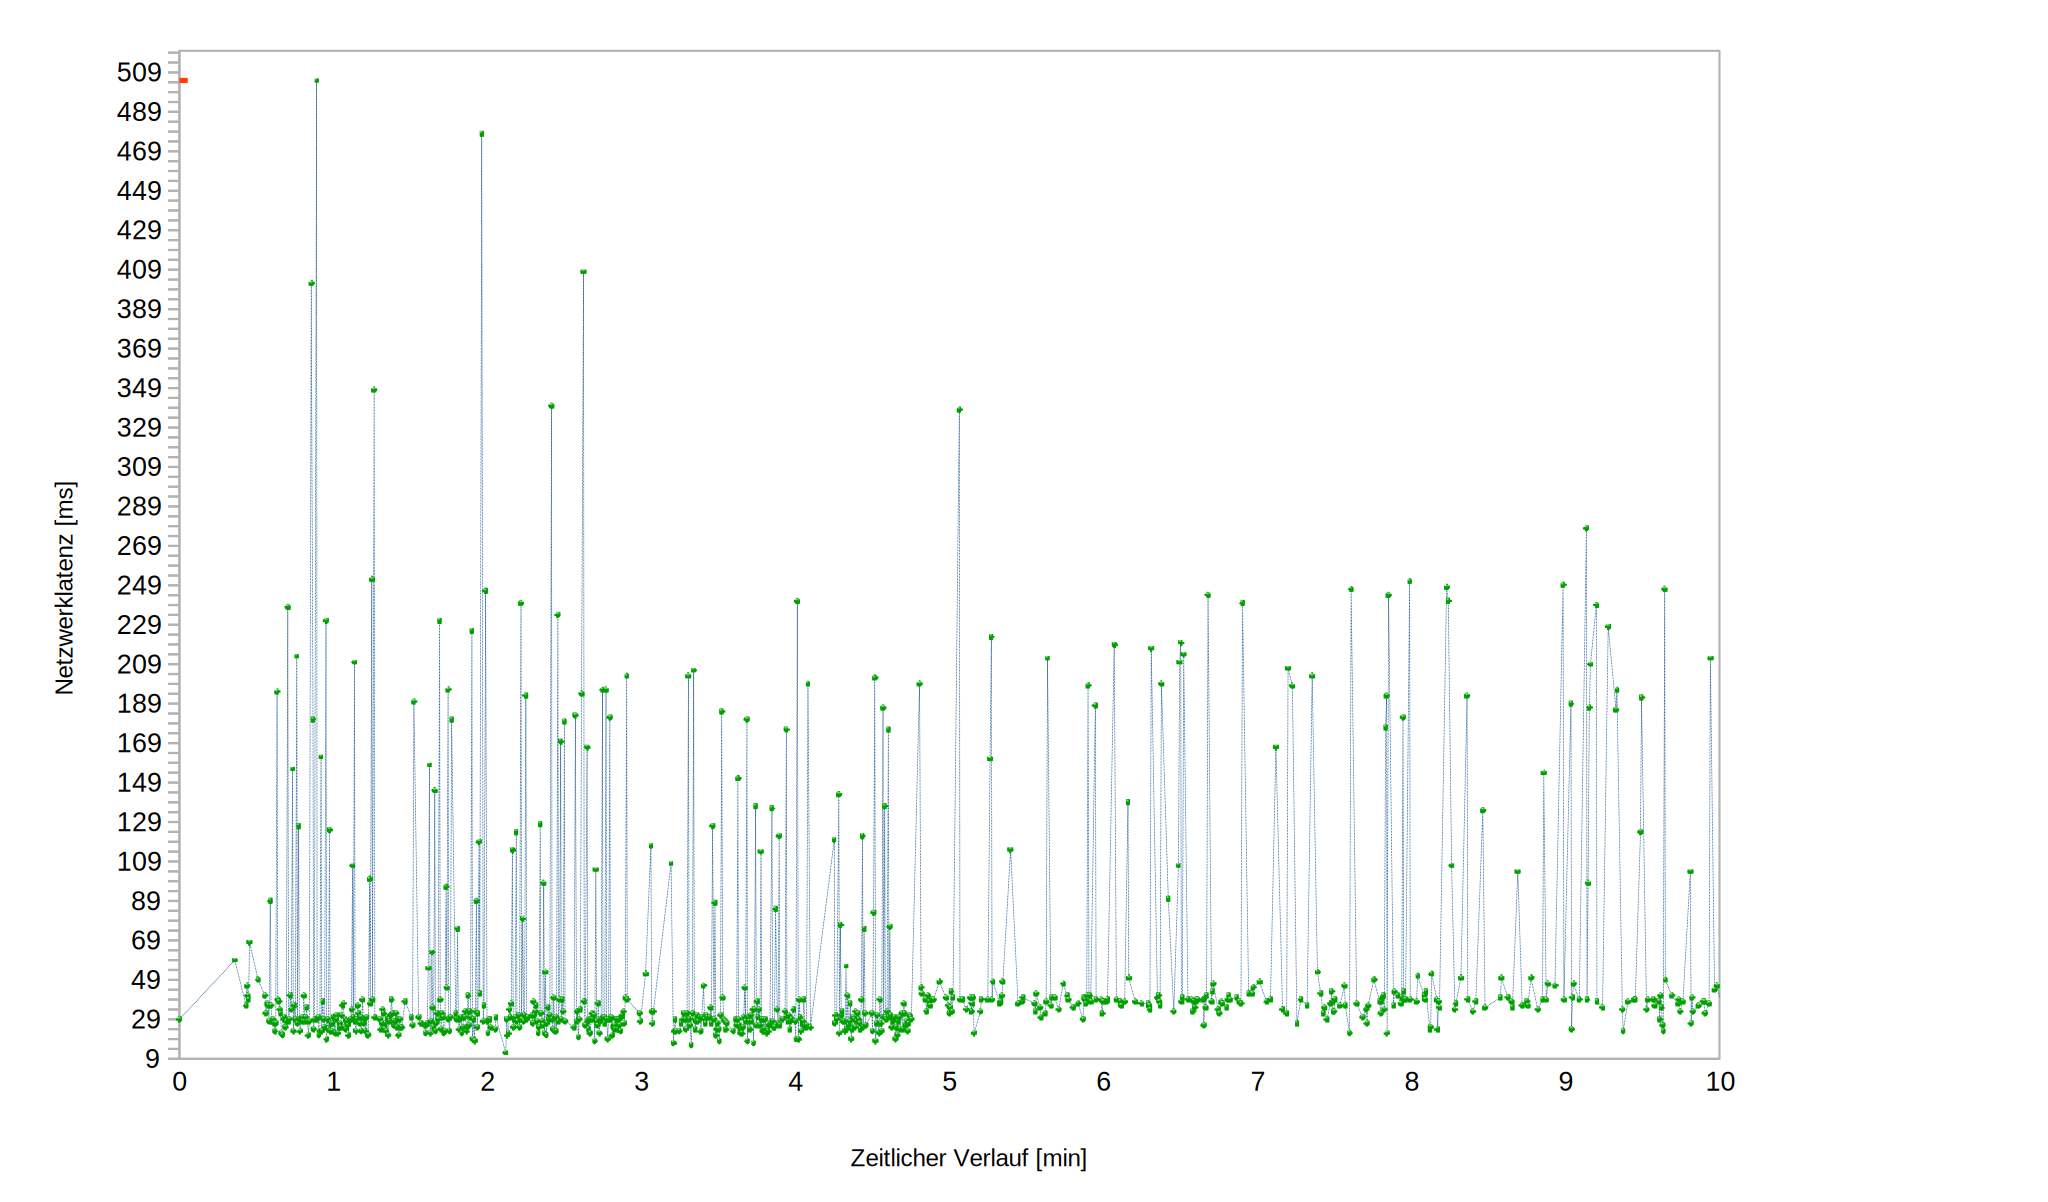
\includegraphics[width=1.04\textwidth]{images/ergebnisse/ROS_App_mit_Netzwerksimulation_und_hohe_Auslastung}
	\caption[Zeitlicher Latenzverlauf der ROS-Kommunikation des \quoteMark{WidowX 200}-Lernroboters (mit Netzwerksimulation, hohe Netzwerkauslastung)]{Zeitlicher Latenzverlauf der ROS-Kommunikation des \quoteMark{WidowX 200}-Lernroboters (mit Netzwerksimulation, hohe Netzwerkauslastung)\\Quelle: Eigene Ausarbeitung}
	\label{fig:measurement_robot_ros_with_network_simulation_high_network_traffic}
\end{figure}
\FloatBarrier

% catkin build -DCMAKE_BUILD_TYPE=Release --cmake-args -DCMAKE_CXX_FLAGS="-DCOMMUNICATION_MEASUREMENT -DMEASUREMENT"
% interbotix_communication_measurement.csv

% für ROS: ein Testnetzwerk aufbauen unterschiedliche Latenzen testen
% Best Case: keine Latenzen
% Worst Case: Übertragen von größeren Datenmengen über ROS (z.B. Kamerabilder, …)

% vom Übertragen des Befehls an die Steuerungseinheit bis der Roboter die Bewegung durchführt
%vom Übertragen des Befehls über TCP/IP bis zur Steuerungseinheit
%vom Durchführen der Geste bis zum erfolgreichen Erkennen von unterschiedlichen Gesten. Unterschiedliche Gesten können mitunter z.T. mehr oder weniger Zeit beanspruchen je nach Komplexität der Geste.


\section{Genauigkeit der Zielpositionen}
Zur Genauigkeitsmessung der Zielpositionen werden diese im Simulator Gazebo durchgeführt. In der Simulationsumgebung wurde ein virtueller Raum erschaffen, in welchem die Zielpositionen bereits genau vordefiniert sind. Die ermittelten Positionen können daraufhin mit den exakten Positionen verglichen werden um so genaue Differenzen bestimmen zu können.

Für diesen Testfall wurde die Roboter-Gesten-Anwendung und deren Abhängigkeiten mittels der Flags \quoteMark{MEASUREMENT} und \quoteMark{POSITION\_MEASUREMENT}, welche im Anhang \ref{appendix1.2:Installation_und_Konfiguration_der_Pakete} aufgezeigt werden, kompiliert.

\textcolor{red}{TODO}

%Im Vergleich zu einer anderen Eingabemethode%\\
%PS3-Controller: https://www.trossenrobotics.com/widowx-200-robot-arm.aspx

% Wie genau kommt man ans gewünschte Ziel? (Einheit: mm)
% Wie viele Korrekturen braucht ein Proband um am nächsten ans gewünschte Ziel zu kommen?

% In einer realen Umgebung nur mit Ungenauigkeiten messbar
%In einer Simulationsumgebung (z.B. Gazebo) kann die Distanz genau und automatisiert gemessen werden
%Visualisierung:
%  *Diagramme
%  *    Mittelwert, die Standardabweichung, Varianz, ...

\begin{figure}[htb]
	\centering
	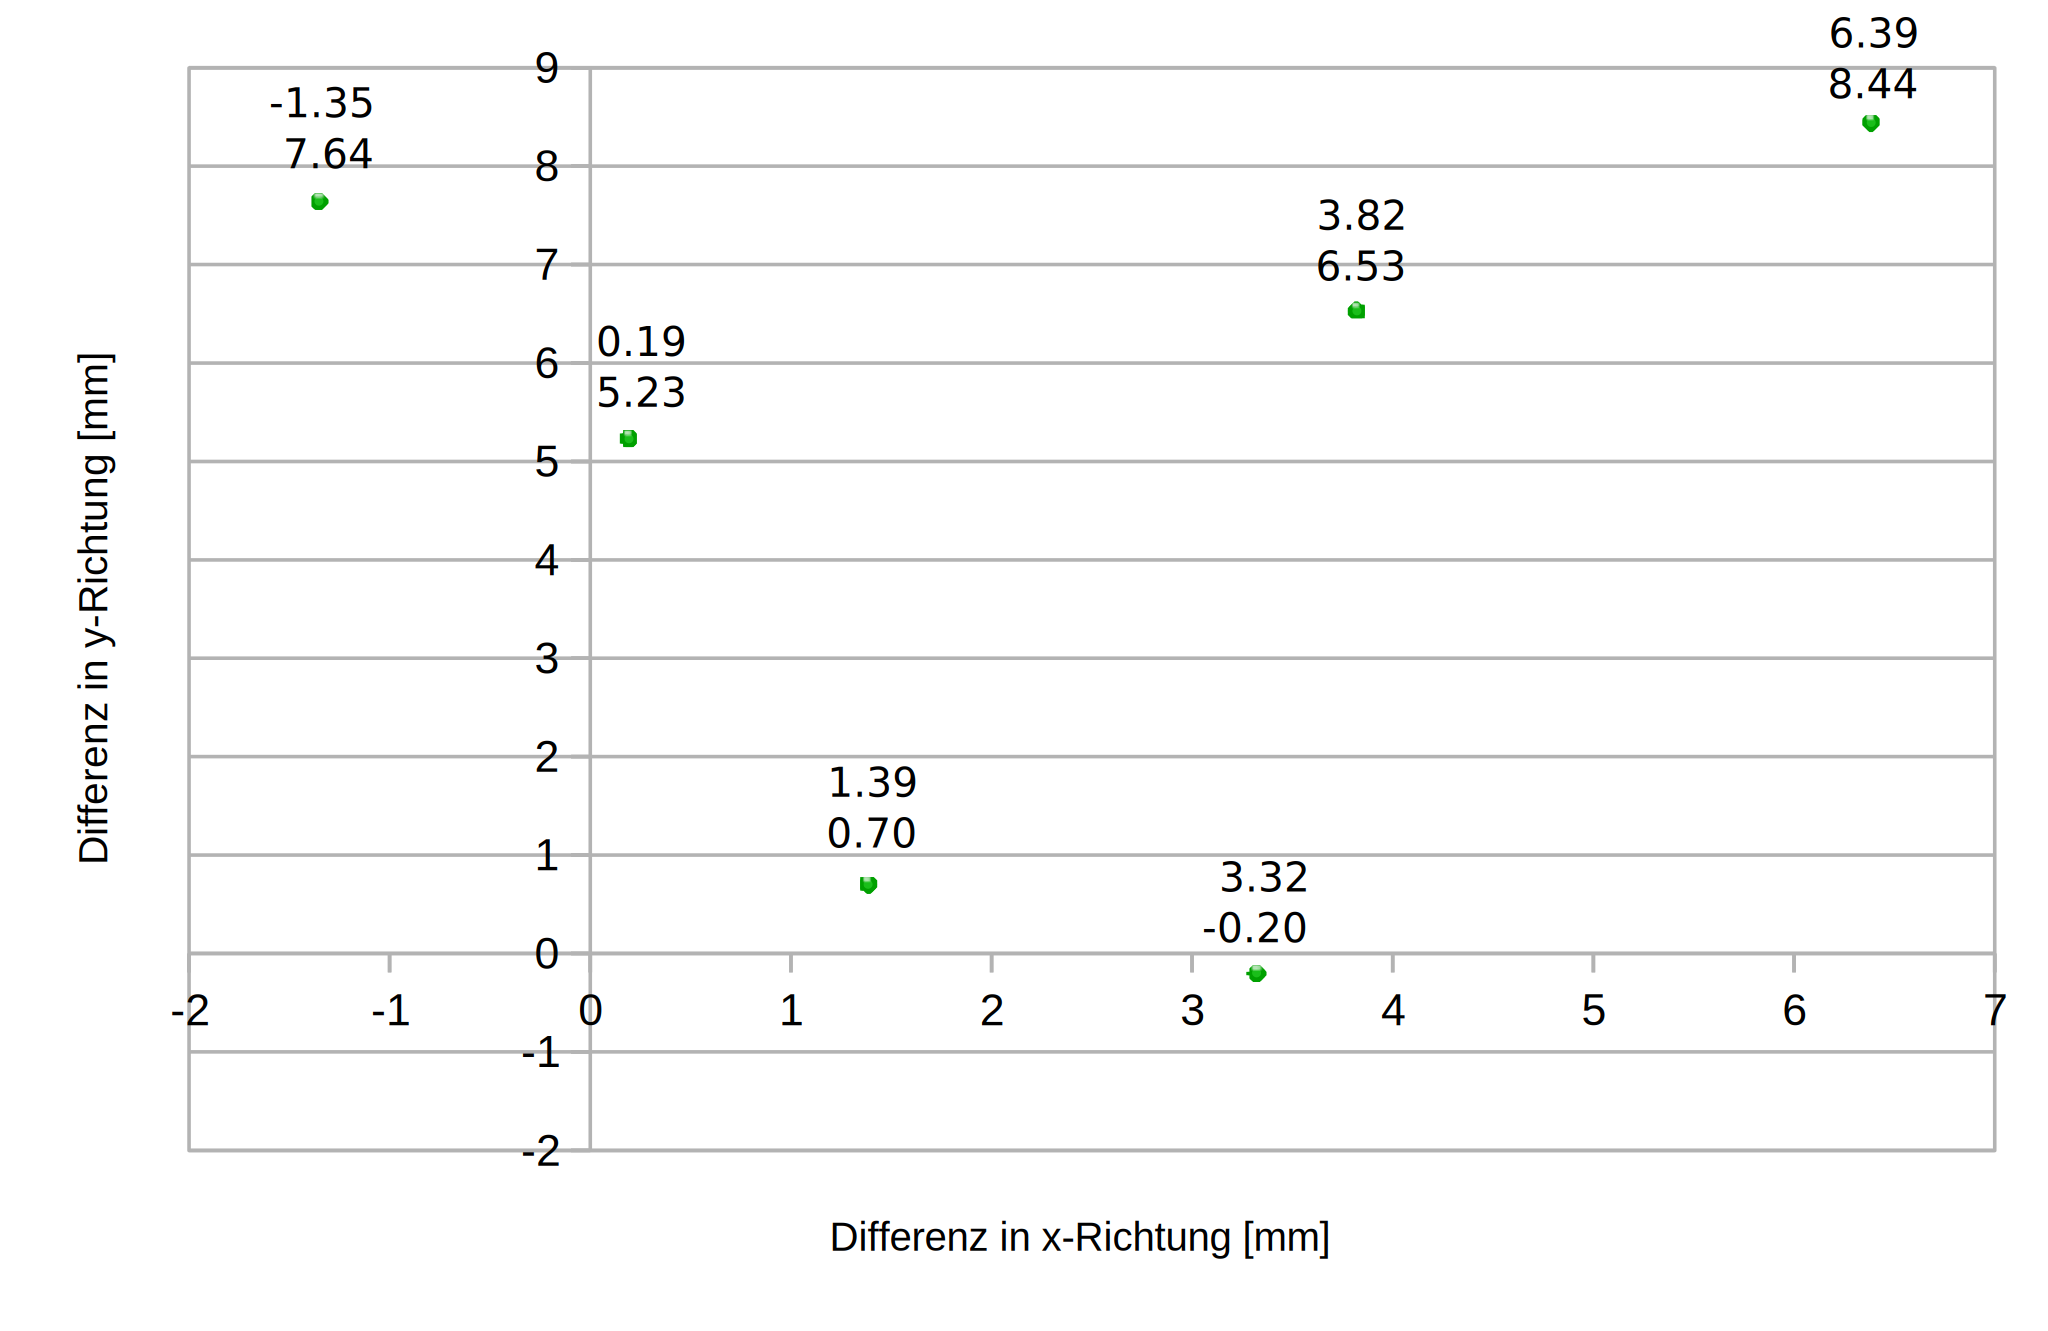
\includegraphics[width=0.88\textwidth]{images/ergebnisse/Differenzen_beim_Teachen_mit_Gesten}
	\caption[Positionsdifferenzen beim Teachen mit der Roboter-Gesten-Anwendung]{Positionsdifferenzen beim Teachen mit der Roboter-Gesten-Anwendung\\Quelle: Eigene Ausarbeitung}
	\label{fig:measurement_teaching_positions}
\end{figure}
\FloatBarrier

\begin{figure}[htb]
	\centering
	\includegraphics[width=0.88\textwidth]{images/ergebnisse/Betrag_der_Fehlerquadrate}
	\caption[Betrag der Fehlerquadrate beim Teachen mit der Roboter-Gesten-Anwendung]{Betrag der Fehlerquadrate beim Teachen mit der Roboter-Gesten-Anwendung\\Quelle: Eigene Ausarbeitung}
	\label{fig:measurement_teaching_positions}
\end{figure}
\FloatBarrier

\section{Genauigkeit der Gestenerkennung}
% Wie viele Versuche benötigt ein Proband bis seine Gesten erkannt werden?

% \section{Ergonomie \& User Experience}
% Verbessert dieser Ansatz die Ergonomie des Teachen in eine positive Richtung?
% Ist es angenehmer diese NUI-Methode zu verwenden als ein herkömmliches Teach Pendant?
% Kann ich über eine längere Zeitspanne, wie z.B. 30 Minuten, einen Roboter teachen?
% Wie schnell bin ich erschöpft im Gegensatz zu einem herkömmlichen Teach Pendant?
% Wie schnell erlernt man die Gesten?
% Wie einprägsam sind die Gesten?
% Sind die Gesten gut geeignet um einen Roboter zu steuern oder sind diese zu schwammig oder zu ähnlich und werden daher auch oft verwechselt?
%   * Können diese im besten Fall nur schwer unbeabsichtigt durchgeführt werden und fälschlicherweise nicht z.B. als kulturelle Geste erkannt werden?
%   * Gibt es wenige Überschneidungen mit bereits definierten Gesten, sodass diese nicht unbeabsichtigt durchgeführt werden können?
%   * Sind diese leicht anzuwenden, sodass das System die Geste im besten Fall beim ersten Mal erkennt?

% Erkennungsrate der Gestenerkennung

\textcolor{red}{TODO:\\
Wie gut ist das System einsetzbar? UX\\
Bewertung der Ergonomie über längere Zeitdauer (sehr subjektiv, jedoch aber versuchen die Ergebnisse auf die Allgemeinheit zu bezienen)\\
Während dem Teachen bewegt man sich oft um zu sehen ob der Endeffektor an der richtigen Stelle ist. Mit einer fest angebrachten Azure Kinect ist es daher schwer den eigenen Blickwinkel zu ändern\\
reflexartige und unbeabsichtigte Bewegungen\\
Beim Teachen steht man normalerweise um den Roboter ordnungsgemäß und vollständig sehen zu können
% siehe 3.4.3 Auswahl anhand der Ergonomie
}

% muss nicht auf die Körpergröße eingestellt werden, da der Field of View sehr groß ist

% Kann ich über eine längere Zeitspanne, wie z.B. 30 Minuten, einen Roboter teachen? Wie schnell bin ich erschöpft im Gegensatz zu einem herkömmlichen Teachpendant? Wie schnell lernt man die Gesten? Sind die Gesten gut geeignet um einen Roboter zu steuern oder sind diese zu schwammig oder zu ähnlich und werden daher auch oft verwechselt?


\chapter{Zusammenfassung \& Ausblick}
\section{Zusammenfassung}

% Azure Kinect: 
%    Stärken der Kinect: Keine Notwendigkeit einer Kalibrierpose, Posenberechnung ohne getragene Hardware
% Problem: immer in Richtung der Azure Kinect schauen -> diese ist statisch

\section{Ausblick}

% ROS ist nicht das Allheilmittel sonder eine mögliche Implementierung die sich erst noch im industriellen Einsatz behaupten muss über die Jahre \cite{noauthor_why_dont_we_use_ros_nodate}

% Was könnte in Zukunft besser gemacht werden?

% Gibt es bessere Alternativen?

% Gibt es weiterführende Themen, welche behandelt werden könnten?


\textcolor{red}{
Weiteres Forschungspotenzial im Bereich der Sicherheit und Ergonomie würde vermutlich zudem in smarten Fußeinlagesohlen bestehen, da hierdurch die Hände zur Gestensteuerung frei bleiben würden. Zudem wäre es womöglich machbar sehr schnelle und reflexartige Druckverteilungen und Bewegungen zu Erkennen und den Industrieroboter bei dieser Art von Bewegung zu stoppen, wenn zu wenig oder kein Druck auf den Sohlen gemessen würde. Dieser Umstand könnte mehrere Gründe haben, da z.B. die Sohlen abgezogen wurden oder die bedienende Person ungewollt auf dem Boden liegt. Das Starten der Gestenerkennung könnte womöglich auch durch eine korrekt ausgeführte Kombination aus Fußbewegungen realisiert werden. --> TODO: Quelle; Vergleich zu Plattform fürs Teachen\newline
\newline
Eine andere Möglichkeit würde darin bestehen einen smarten Handschuh zu verwenden, welcher zu schnelle Bewegungen erkennt und die Bewegung des Industrieroboters anhält. -> TODO: Quelle
}


%\begin{minipage}{\textwidth} % on same page
%	\clearpage
%	\phantomsection
%	\addcontentsline{toc}{chapter}{Abbildungsverzeichnis}
%	\listoffigures
	
	%\clearpage
	%\phantomsection
	%\addcontentsline{toc}{chapter}{Tabellenverzeichnis}
	%\listoftables
	
%	\clearpage
%	\phantomsection
%	\addcontentsline{toc}{chapter}{Listings}
%	\lstlistoflistings
%\end{minipage}

\appendix
\chapter{Anhang}  % evtl. ersetzen mit \chapter*{Anhang}
\addcontentsline{toc}{chapter}{Anhang}
\section{Einrichtung des Testsystems}\label{appendix1:Einrichtung_des_Testsystems}
Zur Einrichtung des Testsystems wird zuallererst ein Linux-Container erstellt, welcher ein einfaches und schnelles Deployen auf unterschiedlichen Linux-Distributionen ermöglicht. Zum Hosten des Linux-Containers wird in dieser Installationsanleitung Ubuntu 20.04 Focal Fossa verwendet, welches eine LTS-Version von Ubuntu darstellt. Nach der Einrichten des Linux-Containers können die benötigten Pakete in dieser neu erstellten Umgebung installiert und daraufhin entsprechend konfiguriert werden. Der vorkonfigurierte Linux-Container ist als Datei \quoteMark{ros-tir.tar.gz} auch auf dem Begleitmedium im Verzeichnis \quoteMark{Linux-Container/} vorzufinden. Dabei ist jedoch zu beachten, dass auf dem Host-System dennoch ein paar wenige Konfigurationsschritte für das Host-System durchgeführt werden müssen. Die Schritte für den Linux-Container können hingegen mit dem vorkonfigurierten Linux-Container übersprungen werden.

\subsection{Erstellen des Linux-Containers}
Für die Installation der Linux-Container-Tools werden Administratorrechte auf dem Zielsystem benötigt. Die benötigten Installationsschritte zum Einrichten des Linux-Containers sind wie folgt \cite{lxd_blog_nodate}.

\begin{enumerate}[label*=\arabic*.]
    \item LXD 4.0 installieren:\
        \begin{lstlisting}[style=bash]
sudo snap install lxd
        \end{lstlisting}
    bzw.
        \begin{lstlisting}[style=bash]
sudo apt install lxd
        \end{lstlisting}

    \item LXD mit den Standardeinstellungen initialisieren:\
        \begin{lstlisting}[style=bash]
lxd init
        \end{lstlisting}

    \item Den derzeitigen User zur LXD-Gruppe hinzufügen:\
        \begin{lstlisting}[style=bash]
sudo adduser $(whoami) lxd
        \end{lstlisting}
        Logout \& Login durchführen oder mittels des folgenden Befehls den User im Terminal neu anmelden.
        \begin{lstlisting}[style=bash]
su - $(whoami)
        \end{lstlisting}

    \item Erstellen des Linux-Containers:\\
        Der Linux-Container wird mit dem folgenden Befehl im Default-Linux-Container-Pool erstellt. Der Platzhalter \quoteMark{<container name>} muss durch einen entsprechenden Namen für den Linux-Container ersetzt werden.
        \begin{lstlisting}[style=bash]
CONTAINER_NAME="<container name>"
lxc init ubuntu:18.04 $CONTAINER_NAME
        \end{lstlisting}
        Mit der Option \quoteMark{-s} kann ein anderer Linux-Container-Pool ausgewählt werden.
        \begin{lstlisting}[style=bash]
lxc init ubuntu:18.04 $CONTAINER_NAME -s <container pool name>
        \end{lstlisting}

    \item Die Eigenschaften des Image des neu erstellten Linux-Containers können mit dem folgenden Befehl eingesehen werden:\
        \begin{lstlisting}[style=bash]
lxc storage list
        \end{lstlisting}

    \item Dem Linux-Container erlauben den X11-Traffic weiterzuleiten:
        \begin{enumerate}[label*=\arabic*.]
            \item Die Datei \quoteMark{gui-profile.yaml} mit dem folgenden Inhalt erstellen:
                \begin{lstlisting}[language=yaml]
config:
  environment.DISPLAY: :0
  raw.idmap: both 1000 1000
  user.user-data: |
    #cloud-config
    package_upgrade: true
    packages:
      - x11-apps
      - mesa-utils
      - pulseaudio
    runcmd:
      - 'sed -i "s/; enable-shm = yes/enable-shm = no/g" /etc/pulse/client.conf'
      - 'echo export PULSE_SERVER=unix:/tmp/.pulse-native | tee --append /home/ubuntu/.profile'
description: GUI LXD profile
devices:
  PASocket:
    path: /tmp/.pulse-native
    source: /run/user/1000/pulse/native
    type: disk
  X0:
    path: /tmp/.X11-unix/X0
    source: /tmp/.X11-unix/X0
    type: disk
  mygpu:
    type: gpu
name: gui
used_by:
                \end{lstlisting}

                \item Bei der Erstellung der Datei \quoteMark{gui-profile.yaml} ist zu beachten, dass die IDs im Eintrag \quoteMark{raw.idmap: both 1000 1000} folgende Bedeutung haben:
                    \begin{lstlisting}[language=yaml]
raw.idmap: both <host user id> <user id in container>
                    \end{lstlisting}

                    \begin{tabular}{|>{\raggedright\arraybackslash}p{0.18\textwidth}|>{\raggedright\arraybackslash}p{0.65\textwidth}|}
                        \hline
                        <host user id>: & Die User-ID, welche zum Starten des Linux-Containers verwendet wird.\\
                        \hline
                        <user id in container>: & Die User-ID des Users innerhalb des Linux-Containers. Normalerweise ist dies die User-ID 1000, da der erste User, welcher im Linux-Container eingerichtet wird, standardmäßig die User-ID 1000 erhält.\\
                        \hline
                    \end{tabular}\\

                \item Das Profil kann daraufhin über die Datei \quoteMark{gui-profile.yaml} geladen werden:
                    \begin{lstlisting}[style=bash]
lxc profile create gui
cat gui-profile.yaml | lxc profile edit gui
                    \end{lstlisting}

                \item Abschließend muss das Profil dem neu erstellten Linux-Container zugewiesen werden:
                    \begin{lstlisting}[style=bash]
lxc profile add $CONTAINER_NAME gui
                    \end{lstlisting}
        \end{enumerate}

% Debugging "Cloud-config" with:
% /var/log/cloud-init-output.log
% lxc console ros-tir --show-log

    \item Den Linux-Container starten und eine Shell im Linux-Container öffnen:
        \begin{lstlisting}[style=bash]
lxc start $CONTAINER_NAME
lxc exec $CONTAINER_NAME -- sudo --user ubuntu --login
        \end{lstlisting}

    \item Um Rendering-Probleme zu vermeiden sollten die neuesten Treiber im Linux-Container installiert werden:
        \begin{lstlisting}[style=bash]
sudo add-apt-repository ppa:oibaf/graphics-drivers -yn
sudo apt upgrade -y
        \end{lstlisting}

    \item Um die durchgeleitete Grafikkarte zu testen muss der Linux-Container neu gestartet werden! Anschließend müssen die folgenden Befehle eingegeben werden:
        \begin{lstlisting}[style=bash]
lspci | grep VGA
        \end{lstlisting}
        bzw.
        \begin{lstlisting}[style=bash]
sudo apt-get install glmark2
glmark2
        \end{lstlisting}

        \begin{redbox}{Wichtig:}
            Anstatt \quoteMark{llvmpipe} sollte die jeweilige verbaute Grafikkarte angezeigt werden.
        \end{redbox}

    \item Für die Soundausgabe sollte PulseAudio getestet werden. Es sollte beim Ausführen des folgenden Befehls ein Rauschen zu hören sein:
        \begin{lstlisting}[style=bash]
pacat < /dev/urandom
        \end{lstlisting}

    \item Von Zeit zu Zeit sollte auf dem Host-System ein Backup vom Linux-Container erstellt werden:
        \begin{lstlisting}[style=bash]
lxc export $CONTAINER_NAME ${CONTAINER_NAME}.tar.gz
        \end{lstlisting}

        bzw. zum Erstellen eines Snapshots

        \begin{lstlisting}[style=bash]
lxc snapshot $CONTAINER_NAME snap01
lxc publish ${CONTAINER_NAME}/snap01 --alias <new-alias>
lxc image export <new-alias> ${CONTAINER_NAME}.tar.gz
        \end{lstlisting}

    \item Das Backup kann auf dem Host-System mittels des folgenden Befehls zurückgespielt werden:
        \begin{redbox}{Wichtig:}
            Beim Import des Linux-Containers muss sichergestellt werden, dass zuvor alle mit dem Linux-Container verknüpften Linux-Container-Profile vorhanden sind, da es ansonsten zu Import-Fehlern kommt.
        \end{redbox}

        \begin{lstlisting}[style=bash]
lxc import <new-alias> ${CONTAINER_NAME}.tar.gz
        \end{lstlisting}

        bzw. der Snapshot

        \begin{lstlisting}[style=bash]
lxc image import ${CONTAINER_NAME}.tar.gz --alias <new-alias>
        \end{lstlisting}
\end{enumerate}


\subsection{Installation \& Konfiguration der Pakete}\label{appendix1.2:Installation_und_Konfiguration_der_Pakete}
Mit der zuvor installierten \quoteMark{Ubuntu 20.04 Focal Fossa}-Umgebung können nun die für diese Arbeit benötigten Pakete innerhalb dieser Umgebung installiert und konfiguriert werden.

\begin{enumerate}[label*=\arabic*.]
    \item Installation von ROS 1:\\
    Zur Nutzung von ROS 1 muss ROS Melodic Morenia installiert werden. Die Installationsanleitung kann man hierzu der offiziellen ROS-Webseite (\href{http://wiki.ros.org/melodic/Installation/Ubuntu}{http://wiki.ros.org/melodic/\\Installation/Ubuntu}) entnehmen. Bei der Installation des ROS-Pakets muss das \quoteMark{ros-melodic-desktop-full}-Paket mit dem folgenden Befehl installiert werden.

        \begin{lstlisting}[style=bash]
sudo apt install ros-melodic-desktop-full
        \end{lstlisting}

    \item Installation des WidowX 200:
        \begin{enumerate}[label*=\arabic*.]
            \item Hierzu müssen zuvor die benötigten Abhängigkeiten installiert werden:

                \begin{lstlisting}[style=bash]
sudo apt install ros-melodic-robot-state-publisher ros-\
melodic-rqt-plot ros-melodic-joy
                \end{lstlisting}

            \item Anschließend müssen die auf der Webseite \href{https://github.com/Interbotix/interbotix_ros_arms#quickstart}{https://github.com/Interbotix/interbotix\\\_ros\_arms\#quickstart} beschriebenen Schritte 1 bis 6 durchgeführt werden.

            \begin{redbox}{Wichtig:}
                Anstelle des \quoteMark{https://github.com/Interbotix/interbotix\_ros\_arms.git}-Repositories muss, dass für diese Arbeit modifizierte Repository, welches auf dem Begleitmedium im Verzeichnis \quoteMark{Repositories/interbotix\_ros\_arms} beigelegt ist, verwendet werden. Zum Klonen des modifizierten Repositories kann man hierzu den folgenden Befehl verwenden:

                \begin{lstlisting}[style=bash]
git clone <Pfad zum Begleitmedium>/Repositories/interbotix_ros_arms/
                \end{lstlisting}
            \end{redbox}

            \item Danach müssen die folgenden Einstellungen auf dem Host-System durchgeführt werden, damit der unprivilegierte Linux-Container Zugriff auf den Dynamixel U2D2 erhält:

                \begin{lstlisting}[style=bash]
wget https://raw.githubusercontent.com/Interbotix/interbotix_ros_arms/\
master/interbotix_sdk/10-interbotix-udev.rules
sudo cp 10-interbotix-udev.rules /etc/udev/rules.d/
sudo udevadm control --reload-rules && sudo udevadm trigger

lxc config device add $CONTAINER_NAME dynamixel_u2d2_ttydxl unix-char path\
=/dev/ttyDXL required=false
                \end{lstlisting}

            \item Innerhalb des Linux-Containers muss zudem der folgende Befehl ausgeführt werden, um als normaler User auf den Dynamixel U2D2 zugreifen zu können:
                \begin{lstlisting}[style=bash]
echo "# Interbotix WidowX 200
sudo chown $(whoami) /dev/ttyDXL" >> ~/.bashrc
source ~/.bashrc
                \end{lstlisting}
        \end{enumerate}

    \item Testen des WidowX 200:
        \begin{redbox}{Wichtig:}
            \begin{compactitem}
                \item Genügend Abstand einhalten
                \item Den Roboter festschrauben
                \item Beim Beenden der Softwaretools den Roboter festhalten, da dieser ansonsten in sich zusammenfällt.
            \end{compactitem}
        \end{redbox}

        Zum Testen der grundlegenden Funktionalität des WidowX 200 können ein paar spezifische ROS-Befehle an diesen gesendet werden.

        \begin{lstlisting}[style=bash]
roslaunch interbotix_descriptions description.launch robot_name:=wx200 jnt_pub\
_gui:=true

roslaunch interbotix_sdk arm_run.launch robot_name:=wx200

rosservice call /wx200/torque_joints_on

roslaunch interbotix_gazebo gazebo.launch robot_name:=wx200
rosservice call /gazebo/unpause_physics
        \end{lstlisting}

%     \item Wichtige Informationen für ROS bekanntmachen:
%         \begin{lstlisting}[style=bash]
% echo "# ROS
% source /opt/ros/melodic/setup.bash
% source ~/interbotix_ws/devel/setup.bash" >> ~/.bashrc
% source ~/.bashrc
%         \end{lstlisting}

    \item Azure Kinect installieren:
        \begin{enumerate}[label*=\arabic*.]
            \item Außerhalb des Linux-Containers müssen die folgenden Einstellungen erfolgen um die Azure Kinect für den derzeitgen User verfügbar zu machen \cite{microsoftazure-kinect-sensor-sdk_installation_nodate}:

                \begin{lstlisting}[style=bash]
wget https://raw.githubusercontent.com/microsoft/Azure-Kinect-Sensor-SDK/\
develop/scripts/99-k4a.rules
sudo cp 99-k4a.rules /etc/udev/rules.d/
sudo udevadm control --reload-rules && sudo udevadm trigger
                \end{lstlisting}

            \item Außerhalb des Linux-Containers müssen die folgenden Einstellungen erfolgen, damit der unprivilegierte Linux-Container Zugriff auf die Azure Kinect erhält:
                \begin{lstlisting}[style=bash]
lxc config device add $CONTAINER_NAME microsoft_generic_superspeed_usb\
_hub usb vendorid=045e productid=097a
lxc config device add $CONTAINER_NAME microsoft_generic_usb\
_hub usb vendorid=045e productid=097b
lxc config device add $CONTAINER_NAME azure_kinect_depth\
_camera usb vendorid=045e productid=097c
lxc config device add $CONTAINER_NAME azure_kinect_4k\
_camera usb vendorid=045e productid=097d
lxc config device add $CONTAINER_NAME azure_kinect_microphone_\
array usb vendorid=045e productid=097e
                \end{lstlisting}

            \item Den Linux-Container neustarten:
                \begin{lstlisting}[style=bash]
lxc restart $CONTAINER_NAME
                \end{lstlisting}
        \end{enumerate}

    \item Azure Kinect SDKs installieren:
        \begin{enumerate}[label*=\arabic*.]
            \item Microsoft-Paketquelle hinzufügen \cite{microsoftazure-kinect-sensor-sdk_installation_nodate}:
                \begin{lstlisting}[style=bash]
sudo apt install curl
curl https://packages.microsoft.com/keys/microsoft.asc | sudo apt-key add -
sudo apt-add-repository https://packages.microsoft.com/ubuntu/18.04/prod
                \end{lstlisting}

            \item Installieren des Azure Kinect SDKs:
                \begin{lstlisting}[style=bash]
sudo apt install k4a-tools=1.3.*
sudo apt install libk4a1.3-dev
                \end{lstlisting}

                \begin{redbox}{Wichtig:}
                    Zur installierten Version des \quoteMark{k4a-tools}-Pakets muss zudem die jeweilige Development-Version des \quoteMark{libk4a}-Pakets installiert werden:

                    \begin{lstlisting}[style=bash]
sudo apt install libk4a<major>.<minor>-dev
                    \end{lstlisting}

                    Der Befehl könnte z.B. wie folgt aussehen:

                    \begin{lstlisting}[style=bash]
sudo apt install libk4a1.3-dev
                    \end{lstlisting}
                \end{redbox}

            \item Um Paketkollisionen beim Updaten zu verhindern sollte das Paket \quoteMark{k4a-tools} vom Updateprozess ausgeschlossen werden:
                \begin{lstlisting}[style=bash]
sudo apt-mark hold k4a-tools
sudo apt-mark showhold
                \end{lstlisting}

            \item Nun kann das Paket \quoteMark{libk4abt1.0-dev} ohne Paketkollisionen installiert werden:
                \begin{lstlisting}[style=bash]
sudo apt install libk4abt1.0-dev
                \end{lstlisting}
        \end{enumerate}

    \item Azure Kinect Firmware aktualisieren:
        \begin{enumerate}[label*=\arabic*.]
            \item Überprüfen ob die Azure Kinect erkannt wird:
                \begin{lstlisting}[style=bash]
AzureKinectFirmwareTool -l
                \end{lstlisting}

            \item Die Ausgabe sollte in etwa wie folgt aussehen:
                \begin{lstlisting}[style=bash]
 == Azure Kinect DK Firmware Tool ==
Found 1 connected devices:
1: Device "000846393812"
                \end{lstlisting}

            \item Die jeweilige Version der Azure Kinect Firmware von der Webseite \href{https://github.com/microsoft/Azure-Kinect-Sensor-SDK/blob/develop/docs/usage.md#msis}{https://github.\\com/microsoft/Azure-Kinect-Sensor-SDK/blob/develop/docs/usage.md\#msis} herunterladen:
                \begin{lstlisting}[style=bash]
wget https://download.microsoft.com/download/1/9/8/198048e8-63f2-45c6-\
8f96-1fd541d1b4bc/AzureKinectDK_Fw_1.6.102075014.bin
                \end{lstlisting}

            \item Die heruntergeladene Azure Kinect Firmware daraufhin flashen:
                \begin{lstlisting}[style=bash]
AzureKinectFirmwareTool -u AzureKinectDK_Fw_1.6.102075014.bin
                \end{lstlisting}
        \end{enumerate}

    \item Azure Kinect testen:
        \begin{enumerate}[label*=\arabic*.]
            \item Device-Stream testen:
                \begin{lstlisting}[style=bash]
k4aviewer
                \end{lstlisting}

            \item Body Tracking testen:\\
                Die OpenGL-Version, der Grafikkartenname und der eingesetzte Grafikkartentreiber kann mit den folgenden Befehlen abgefragt werden:
                \begin{lstlisting}[style=bash]
sudo apt install mesa-utils
glxinfo | grep -E "Device:|OpenGL version"
                \end{lstlisting}

                Die Ausgabe kann z.B. wie folgt aussehen:
                \begin{lstlisting}[style=bash]
    Device: AMD Radeon RX 5700 XT (NAVI10, DRM 3.35.0, 5.4.0-39-generic,\
 LLVM 10.0.0) (0x731f)
OpenGL version string: 4.6 (Compatibility Profile) Mesa 20.2.0-devel (git\
-c0c03f4 2020-06-27 bionic-oibaf-ppa)
                \end{lstlisting}

                \begin{redbox}{Wichtig:}
                    Für das Body Tracking wird ein Grafikkartentreiber mit mindestens \quoteMark{OpenGL 4.4}- und \quoteMark{OpenGL Compatibility Context}-Unterstützung benötigt. Bei den Open-Source-Mesa-Treibern tritt lauf Stand 29. März 2020 mit dem \quoteMark{k4a-tools}-Paket in der Version 1.3 oder niedriger der Fehler\newline\newline
                    \quoteMark{Shader Error: 0:2(38): error: `gl\_FragColor' undeclared\\0:2(38): error: value of type vec4 cannot be assigned to variable of type error}\newline\newline
                    auf, welcher das Starten der \quoteMark{k4abt\_simple\_3d\_viewer}-Anwendung verhindert.\\

                    Hierzu muss die \quoteMark{simple\_3d\_viewer}-Anwendung mit dem in dieser Arbeit erstellten GLSL-Patch\footnote{\href{https://github.com/microsoft/Azure-Kinect-Samples/commit/15c303fb9a3a6b3a2c54a57cb11996823389595a}{https://github.com/microsoft/Azure-Kinect-Samples/commit/15c303fb9a3a6b3a\\2c54a57cb11996823389595a}}, welcher bereits in den Hauptzweig des \quoteMark{Azure-Kinect-Samples}-Repositories eingepflegt wurde, neukompiliert werden. Getestet wurde das Kompilieren mit der Commit-Version \quoteMark{ac696e4015648dd82dd019e59d94ba169f3c81aa}. Wenn ein Fehler beim Kompilieren auftritt, kann nach dem Klonen des Repositories explizit mit dem folgenden Befehl auf den in dieser Arbeit verwendeten Stand des Repositories zugegriffen werden.
                    \begin{lstlisting}[style=bash]
git checkout ac696e4015648dd82dd019e59d94ba169f3c81aa
                    \end{lstlisting}

                    Zum kompilieren der \quoteMark{simple\_3d\_viewer}-Anwendung müssen die folgenden Schritte eingehalten werden.
                    \newcounter{bt_wichtig}
                    \begin{enumerate}[label=\arabic*.]
                        \item Das \quoteMark{Azure-Kinect-Samples}-Repository klonen:
                            \begin{lstlisting}[style=bash]
git clone --recursive https://github.com/microsoft/Azure\
-Kinect-Samples.git
cd Azure-Kinect-Samples/
                            \end{lstlisting}

                        \item Um einen Kompilierfehler\footnote{\label{fn:pull_request_54}\href{https://github.com/microsoft/Azure-Kinect-Samples/pull/54}{https://github.com/microsoft/Azure-Kinect-Samples/pull/54}} zu vermeiden muss in der Datei \quoteMark{CMakeLists.txt} zwischen \quoteMark{FIND\_PACKAGE(k4a REQUIRED)} und \quoteMark{FIND\_PACKAGE(k4abt REQUIRED)} der Text \quoteMark{FIND\_PACKAGE(k4arecord REQUIRED)} eingefügt werden. Um einen weiteren Kompilierfehler\footref{fn:pull_request_54} zu vermeiden muss zudem in der Datei \quoteMark{CMakeLists.txt} im Verzeichnis \quoteMark{body-tracking-samples/simple\_3d\_viewer/} zwischen \quoteMark{k4abt} und \quoteMark{window\_controller\_3d::window\_controller\_3d} der Text \quoteMark{k4arecord} eingefügt werden.
                        \setcounter{bt_wichtig}{\value{enumiii}}
                    \end{enumerate}
                \end{redbox}

                \begin{redbox}{}
                    \begin{enumerate}[label=\arabic*.]
                        \setcounter{enumiii}{\value{bt_wichtig}}
                        \item Notwendige Pakete zum Kompilieren der \quoteMark{simple\_3d\_viewer}-Anwendung installieren:
                            \begin{lstlisting}[style=bash]
sudo apt install libxi-dev cmake ninja-build
sudo apt install libxrandr-dev libxinerama-dev libxcursor\
-dev libgl-dev # for GLFW
sudo apt install mesa-vulkan-drivers # for Vulkan support in
                                         # GLFW (optional)
                            \end{lstlisting}

                        \item Die \quoteMark{simple\_3d\_viewer}-Anwendung komplieren und ausführbar machen:
                            \begin{lstlisting}[style=bash]
mkdir build
cd build
cmake .. -GNinja
ninja

chmod +x ./bin/simple_3d_viewer
                            \end{lstlisting}
                    \end{enumerate}
                \end{redbox}
%nm -gD /usr/lib/x86_64-linux-gnu/libk4arecord.so | grep -i "k4a_playback"

                Wenn eine Nvidia-GPU verbaut ist, kann die GPU-Beschleunigung eingesetzt werden. Hierzu muss das CUDA-Paket installiert werden:
                \begin{lstlisting}[style=bash]
k4abt_simple_3d_viewer
                \end{lstlisting}

                Daraufhin kann die \quoteMark{simple\_3d\_viewer}-Anwendung mit GPU-Beschleunigung gestartet werden:
                \begin{lstlisting}[style=bash]
k4abt_simple_3d_viewer
                \end{lstlisting}

                bzw.

                \begin{lstlisting}[style=bash]
~/Azure-Kinect-Samples/build/bin/simple_3d_viewer
                \end{lstlisting}

                Wenn keine Nvidia-GPU verbaut ist muss ansonsten der CPU-Modus verwendet werden:
                \begin{lstlisting}[style=bash]
k4abt_simple_3d_viewer CPU
                \end{lstlisting}

                bzw.

                \begin{lstlisting}[style=bash]
~/Azure-Kinect-Samples/build/bin/simple_3d_viewer CPU
                \end{lstlisting}
        \end{enumerate}

    \item Zum Kompilieren der Roboter-Gesten-Anwendung müssen die folgenden Pakete installiert werden:
        \begin{lstlisting}[style=bash]
sudo apt install cmake gdb gcc python python-catkin-tools
        \end{lstlisting}

    \item Source Code kompilieren:\\
        \begin{redbox}{Wichtig:}
            Die Roboter-Gesten-Anwendung wird mit der Option \quoteMark{Release} kompiliert. Dies ist empfehlenswert, wenn die Roboter-Gesten-Anwendung im Produktivbetrieb eingesetzt werden soll. Die Option \quoteMark{Release} kann durch die Option \quoteMark{Debug} ersetzt werden um eine Entwicklerversion mit zusätzlicher Ausgabe zu erhalten. Um eine Version zur Durchführung der in dieser Arbeit erläuterten Messungen zu erhalten wird die Option \quoteMark{Release} und zusätzlich eine der folgenden Optionen für den jeweiligen Testfall verwendet:

            \begin{lstlisting}[style=bash]
--cmake-args -DCMAKE_CXX_FLAGS="-DMEASUREMENT -DGESTURE_MEASUREMENT"
--cmake-args -DCMAKE_CXX_FLAGS="-DMEASUREMENT -DCOMMUNICATION_MEASUREMENT"
--cmake-args -DCMAKE_CXX_FLAGS="-DMEASUREMENT -DPOSITION_MEASUREMENT"
            \end{lstlisting}
        \end{redbox}
        \begin{enumerate}[label*=\arabic*.]
            \item InterbotiX SDK kompilieren:
                \begin{lstlisting}[style=bash]
cd ~/interbotix_ws
rm -rf build devel/
catkin build -DCMAKE_BUILD_TYPE=Release
source ~/.bashrc
                \end{lstlisting}

            \item Den Source Code der Roboter-Gesten-Anwendung auf dem Begleitmedium aus dem Verzeichnis \quoteMark{Repositories/Teach-Industrial-Robots} klonen, Abhängigkeiten installieren und anschließend die Roboter-Gesten-Anwendung kompilieren:
                \begin{lstlisting}[style=bash]
mkdir -p ~/tir_ws/src
cd ~/tir_ws/
catkin build -DCMAKE_BUILD_TYPE=Release
echo "# ROS
source ~/tir_ws/devel/setup.bash" >> ~/.bashrc
source ~/.bashrc

cd ~/tir_ws/src
git clone <Pfad zum Begleitmedium>/Repositories/Teach-Industrial-Robots/

sudo apt install libglm-dev libeigen3-dev rapidjson-dev libk4a1.3\
-dev libk4abt1.0-dev

cd ~/tir_ws
catkin build -DCMAKE_BUILD_TYPE=Release
source ~/.bashrc
                \end{lstlisting}
        \end{enumerate}

    \item Entwicklungsumgebung installieren (optional):
        \begin{enumerate}[label*=\arabic*.]
            \item Temporärer Ordner erstellen:
                \begin{lstlisting}[style=bash]
echo "# Temporary user folder
sudo mkdir -p /run/user/$(id --user)
sudo chown $(whoami) /run/user/$(id --user)" >> ~/.bashrc
source ~/.bashrc
                \end{lstlisting}

            \item VS Code installieren:
                \begin{lstlisting}[style=bash]
sudo snap install code --classic
                \end{lstlisting}

            \item Starten der Entwicklungsumgebung mit dem folgenden Befehl:
                \begin{lstlisting}[style=bash]
code
                \end{lstlisting}

            \item Mittels Strg + P in VS Code das \quoteMark{Quick Open}-Menü öffnen und jeweils eine der folgenden Befehle eingeben um die notwendigen Plugins zu installieren:
                \begin{lstlisting}[style=bash]
ext install ms-vscode.cpptools
ext install ms-vscode.cmake-tools
ext install ms-python.python
ext install ms-iot.vscode-ros
                \end{lstlisting}
        \end{enumerate}

        \item Wenn der Speicherplatz des Linux-Containers zu knapp wird, kann der Speicherplatz des Linux-Containers wie folgt auf dem Host-System vergrößert werden:
            \begin{enumerate}[label*=\arabic*.]
                \item Image des Linux-Containers z.B. um 5 GB vergrößern:
                    \begin{lstlisting}[style=bash]
sudo truncate -s +5G /var/snap/lxd/common/lxd/disks/default.img
                    \end{lstlisting}

                \item Host-System neustarten

                \item Anschließend das Image des Linux-Containers im zuvor erstellten Ordnerpfad \quoteMark{/<mount point>} einhängen und daraufhin die neue Größe des Images eingeben:
                    \begin{lstlisting}[style=bash]
sudo mount /var/snap/lxd/common/lxd/disks/default.img /<mount point>
sudo btrfs filesystem resize maxG /<mount point>
                    \end{lstlisting}
            \end{enumerate}
\end{enumerate}


\subsection{Starten der Roboter-Gesten-Anwendung}
Für die Roboter-Gesten-Anwendung wird der \quoteMark{SCHED\_DEADLINE}-Scheduler eingesetzt, welcher für diese Arbeit feste Echtzeitfähigkeit im 50 ms Bereich garantieren kann.

\begin{figure}[htb]
	\centering
	\includegraphics[width=0.85\textwidth]{images/anhang/sched_deadline}
	\caption[Ablauf von SCHED\_DEADLINE]{Ablauf von SCHED\_DEADLINE\\Quelle: Eigene Darstellung, in Anlehnung an \cite{man_sched7_nodate}}
	\label{fig:sched_deadline}
\end{figure}
\FloatBarrier

Für den \quoteMark{SCHED\_DEADLINE}-Scheduler müssen hierfür die Parameter, welche in Abbildung \ref{fig:sched_deadline} ersichtlich sind, ordnungsgemäß eingestellt werden. Der \quoteMark{Runtime}-Parameter beträgt zur Einhaltung der 50 ms Frist hierbei 50000000 ns, der \quoteMark{Deadline}-Parameter beträgt 50000000 ns und der \quoteMark{Periode}-Parameter beträgt 50000000 ns. Der \quoteMark{Runtime}-Parameter steht hierbei für die maximal benötigte Ausführungszeit der Aufgabe, der \quoteMark{Deadline}-Parameter für die Zeit die die Aufgabe mit überzogener Ausführungszeit maximal benötigen darf und der \quoteMark{Periode}-Parameter für wann die nächste Periode gestartet werden muss \cite{man_sched7_nodate}. Diese Einstellungen wurden im Listing \ref{lst:settings_for_start_script} bei den Bash Variablen \quoteMark{SCHED\_RUNTIME}, \quoteMark{SCHED\_DEADLINE} und \quoteMark{SCHED\_PERIOD} im Start-Script bereits voreingestellt.\\

\begin{lstlisting}[style=bash, caption={Einstellungen des Start-Scripts der Roboter-Gesten-Anwendung}, label={lst:settings_for_start_script}]
USE_ROS_COMMUNICATION=true
USE_SIMULATION=true  # Only usable with "USE_ROS_COMMUNICATION=true"
DO_MEASUREMENT=false  # Only usable with "USE_SIMULATION=false" and
                       # "USE_ROS_COMMUNICATION=true"
SIMULATE_ADDITIONAL_ROS_NODES=false  # Only usable with "DO_MEASUREMENT=true"
ADDITIONAL_ROS_NODES_COUNT=3  # Only usable with "SIMULATE_OTHER_ROS_NODES=true"
LXC_USER_NAME="ubuntu"
LXC_INSTANCE="<container name>"
ADDITIONAL_APP_PARAMETERS="--move-home-at-exit --move-home-at-error"
TEACH_POSITIONS=true  # If "true" positions can be teached. Otherwise the positions
                        # in the file "robot_arm_positions.json" will be executed.
CONFIGURATION_FILE_PATH=""  # Empty for the default file path
                              # ("~/robot_arm_positions.json")
SCHED_RUNTIME=50000000
SCHED_DEADLINE=50000000
SCHED_PERIOD=50000000
\end{lstlisting}\leavevmode\newline\vspace{-1.0em}

Die Roboter-Gesten-Anwendung kann mit dem Start-Script \quoteMark{start\_tir.sh}, welches sich auf dem Begleitmedium im Verzeichnis \quoteMark{Repositories/Teach-Industrial-Robots} befindet, durch das Host-System im Linux-Container gestartet und dem \quoteMark{SCHED\_DEADLINE}-Scheduler zugewiesen werden. Die einstellbaren Optionen des Start-Scripts sind im Listing \ref{lst:settings_for_start_script} ersichtlich. Zum Ausführen des Start-Scripts muss im Listing \ref{lst:settings_for_start_script} der Bash-Variable \quoteMark{LXC\_INSTANCE} der Name des Linux-Containers zugewiesen werden. Die Bash-Variable \quoteMark{USE\_ROS\_COMMUNICA-\\TION} steuert ob die Roboter-Gesten-Anwendung über ROS kommunizieren oder eine direkt Verbindung mit dem Industrieroboter aufbauen soll. Um der Roboter-Gesten-Anwendung mitteilen zu können ob diese im Lern- oder Abspielmodus gestartet werden soll, wird die Bash-Variable \quoteMark{TEACH\_POSITIONS} eingesetzt. Zur Auswahl der verwendeten Positionsdatei kann die Bash-Variable \quoteMark{CONFIGURATION\_FILE\_PATH} mit dem Pfad zur Positionsdatei genutzt werden. Mit der Bash-Variable \quoteMark{USE\_SIMULATION} kann eingestellt werden ob die Anwendung im Simulator gestartet werden soll. Die Bash-Variable \quoteMark{DO\_MEASUREMENT} kann bei Verwendung eines realen Industrieroboters dazu verwendet werden um Messvorraussetzungen, wie z.B. ein simuliertes Netzwerk, bereitzustellen. Zudem kann bei aktivierter \quoteMark{DO\_MEASUREMENT}-Bash-Variable die Bash-Variable \quoteMark{SIMULATE\_ADDITIONAL\_ROS\\\_NODES} aktiviert werden um zusätzlichen Netzwerktraffic zu generieren. Mit der Bash-Variable \quoteMark{ADDITIONAL\_ROS\_NODES\_COUNT} kann bei aktivierter \quoteMark{SIMULATE\_ADD-\\ITIONAL\_ROS\_NODES}-Bash-Variable auch die Anzahl der zu simulierenden ROS-Nodes angegeben werden. Es werden 4K-Kamera-ROS-Nodes simuliert, welche jeweils 4K-Bilder mit 60 FPS per UDP über die Netzwerkschnittstelle transferieren. Um weitere von der Roboter-Gesten-Anwendung unterstützte Parameter anwenden zu können, kann die Bash-Variable \quoteMark{ADDITIONAL\_APP\_PARAMETERS} mit den nachstehenden Parametern modifiziert werden.

\begin{longtable}{|>{\raggedright\arraybackslash}p{0.2\textwidth}|>{\raggedright\arraybackslash}p{0.20\textwidth}|>{\raggedright\arraybackslash}p{0.50\textwidth}|}
\hline
\rowcolor{LightGray} \thead[c]{Kurzschreibweise\\des\\Parameters} & \thead[c]{Ausgeschriebener\\Parameter} & \thead[c]{Beschreibung}\\
\hline
-pfp="\phantom{}<path>" & \texttt{-{}-}positions-file-path="\phantom{}<path>" & Dateipfad zum Speichern oder Laden der aufgezeichneten Positionen \newline (Default-Positionsdateipfad: "\~{}/robot\_arm\_positions.json")\\
\hline
-opf & \texttt{-{}-}overwrite-positions-file & Ermöglicht das Überschreiben der Positionsdatei. Zuvor sollte ein Backup der Positionsdatei gemacht werde um Datenverlust zu vermeiden.\\
\hline
-rrp & \texttt{-{}-}repeat-recorded-positions & Die aufgezeichneten Positionen aus der Positionsdatei wiederholen lassen\\
\hline
-tp & \texttt{-{}-}teach-positions & Positionen lernen\\
\hline
-rn="\phantom{}<name>" & \texttt{-{}-}robot-name="\phantom{}<name>" & Name des Roboters\newline (Default: "wx200")\\
\hline
-rm="\phantom{}<model>" & \texttt{-{}-}robot-model="\phantom{}<model>" & Robotermodell\newline (In der Regel der Name des Roboters\newline Default: "wx200")\\
\hline
-ur & \texttt{-{}-}use-ros & Mittels ROS oder einer direkten Verbindung mit dem Industrieroboter kommunizieren\\
\hline
-mhaex & \texttt{-{}-}move-home-at-exit & Beim Beenden der Anwendung in die Ausgangsposition zurückfahren\\
\hline
-mhaer & \texttt{-{}-}move-home-at-error & Bei einem Fehler der Anwendung in die Ausgangsposition zurückfahren\\
\hline
 & \texttt{-{}-}help & Zeigt die Hilfe\\
\hline
\end{longtable}


% Literaturverzeichnis:
\clearpage
\phantomsection
\addcontentsline{toc}{chapter}{Literaturverzeichnis}
\printbibliography


\chapter*{Eidesstattliche Erklärung}
\addcontentsline{toc}{chapter}{Eidesstattliche Erklärung}
Ich erkläre hiermit an Eides statt, dass ich die vorliegende Masterarbeit selbstständig und ohne Benutzung anderer als der angegebenen Hilfsmittel angefertigt habe. Die aus fremden Quellen direkt oder indirekt übernommenen Stellen sind als solche kenntlich gemacht. Die Arbeit wurde bisher weder in gleicher noch in ähnlicher Form einer anderen Prüfungsbehörde vorgelegt und auch noch nicht veröffentlicht.

\vspace{3cm}
\noindent
Dornbirn, am \today %[Tag. Monat Jahr anführen]
\hfill Helmut Rhomberg %[Vor- und Nachname Verfasser/in]


\end{document}
